% ---
% Arquivo com a metodologia do Trabalho de Conclusão de Curso dos alunos
% Gabriel Takaoka Nishimura, Felippe Demarqui Ramos e Vivian Kimie Isuyama 
% da Escola Politécnica da Universidade de São Paulo
% ---
	% ---
	\chapter{Metodologia}\label{cap-metodologia}
	% ---
	
	Nesse capítulo são discorridas as escolhas da \texttt{norma 802.15.7}, \textit{hardware} e \texttt{software}.
	
	% ---
	\section{Planejamento}\label{sec-planejamento}
	% ---
	
	% ---
	\subsection{Estrutura Analítica do Projeto}\label{subsec-eap}
	% ---
	
	A Estrutura Analítica do Projeto é uma ferramenta de gerenciamento que divide as principais entregas de um projeto. Cada entrega deve ser subdividida em tarefas até que sejam obtidos pacotes de trabalho, para que se estime recursos e tempo demandados. Neste projeto, foram definidas a partir da EAP as fases de trabalho. Observa-se que existe uma fase de gerenciamento, três fases de desenvolvimento e uma fase final para o encerramento.
	
	
	\begin{figure}[h!]
		\caption{\label{fig_eap} Estrutura Analítica do Projeto Light Cyber }
		\centering
		\scalebox{.96}{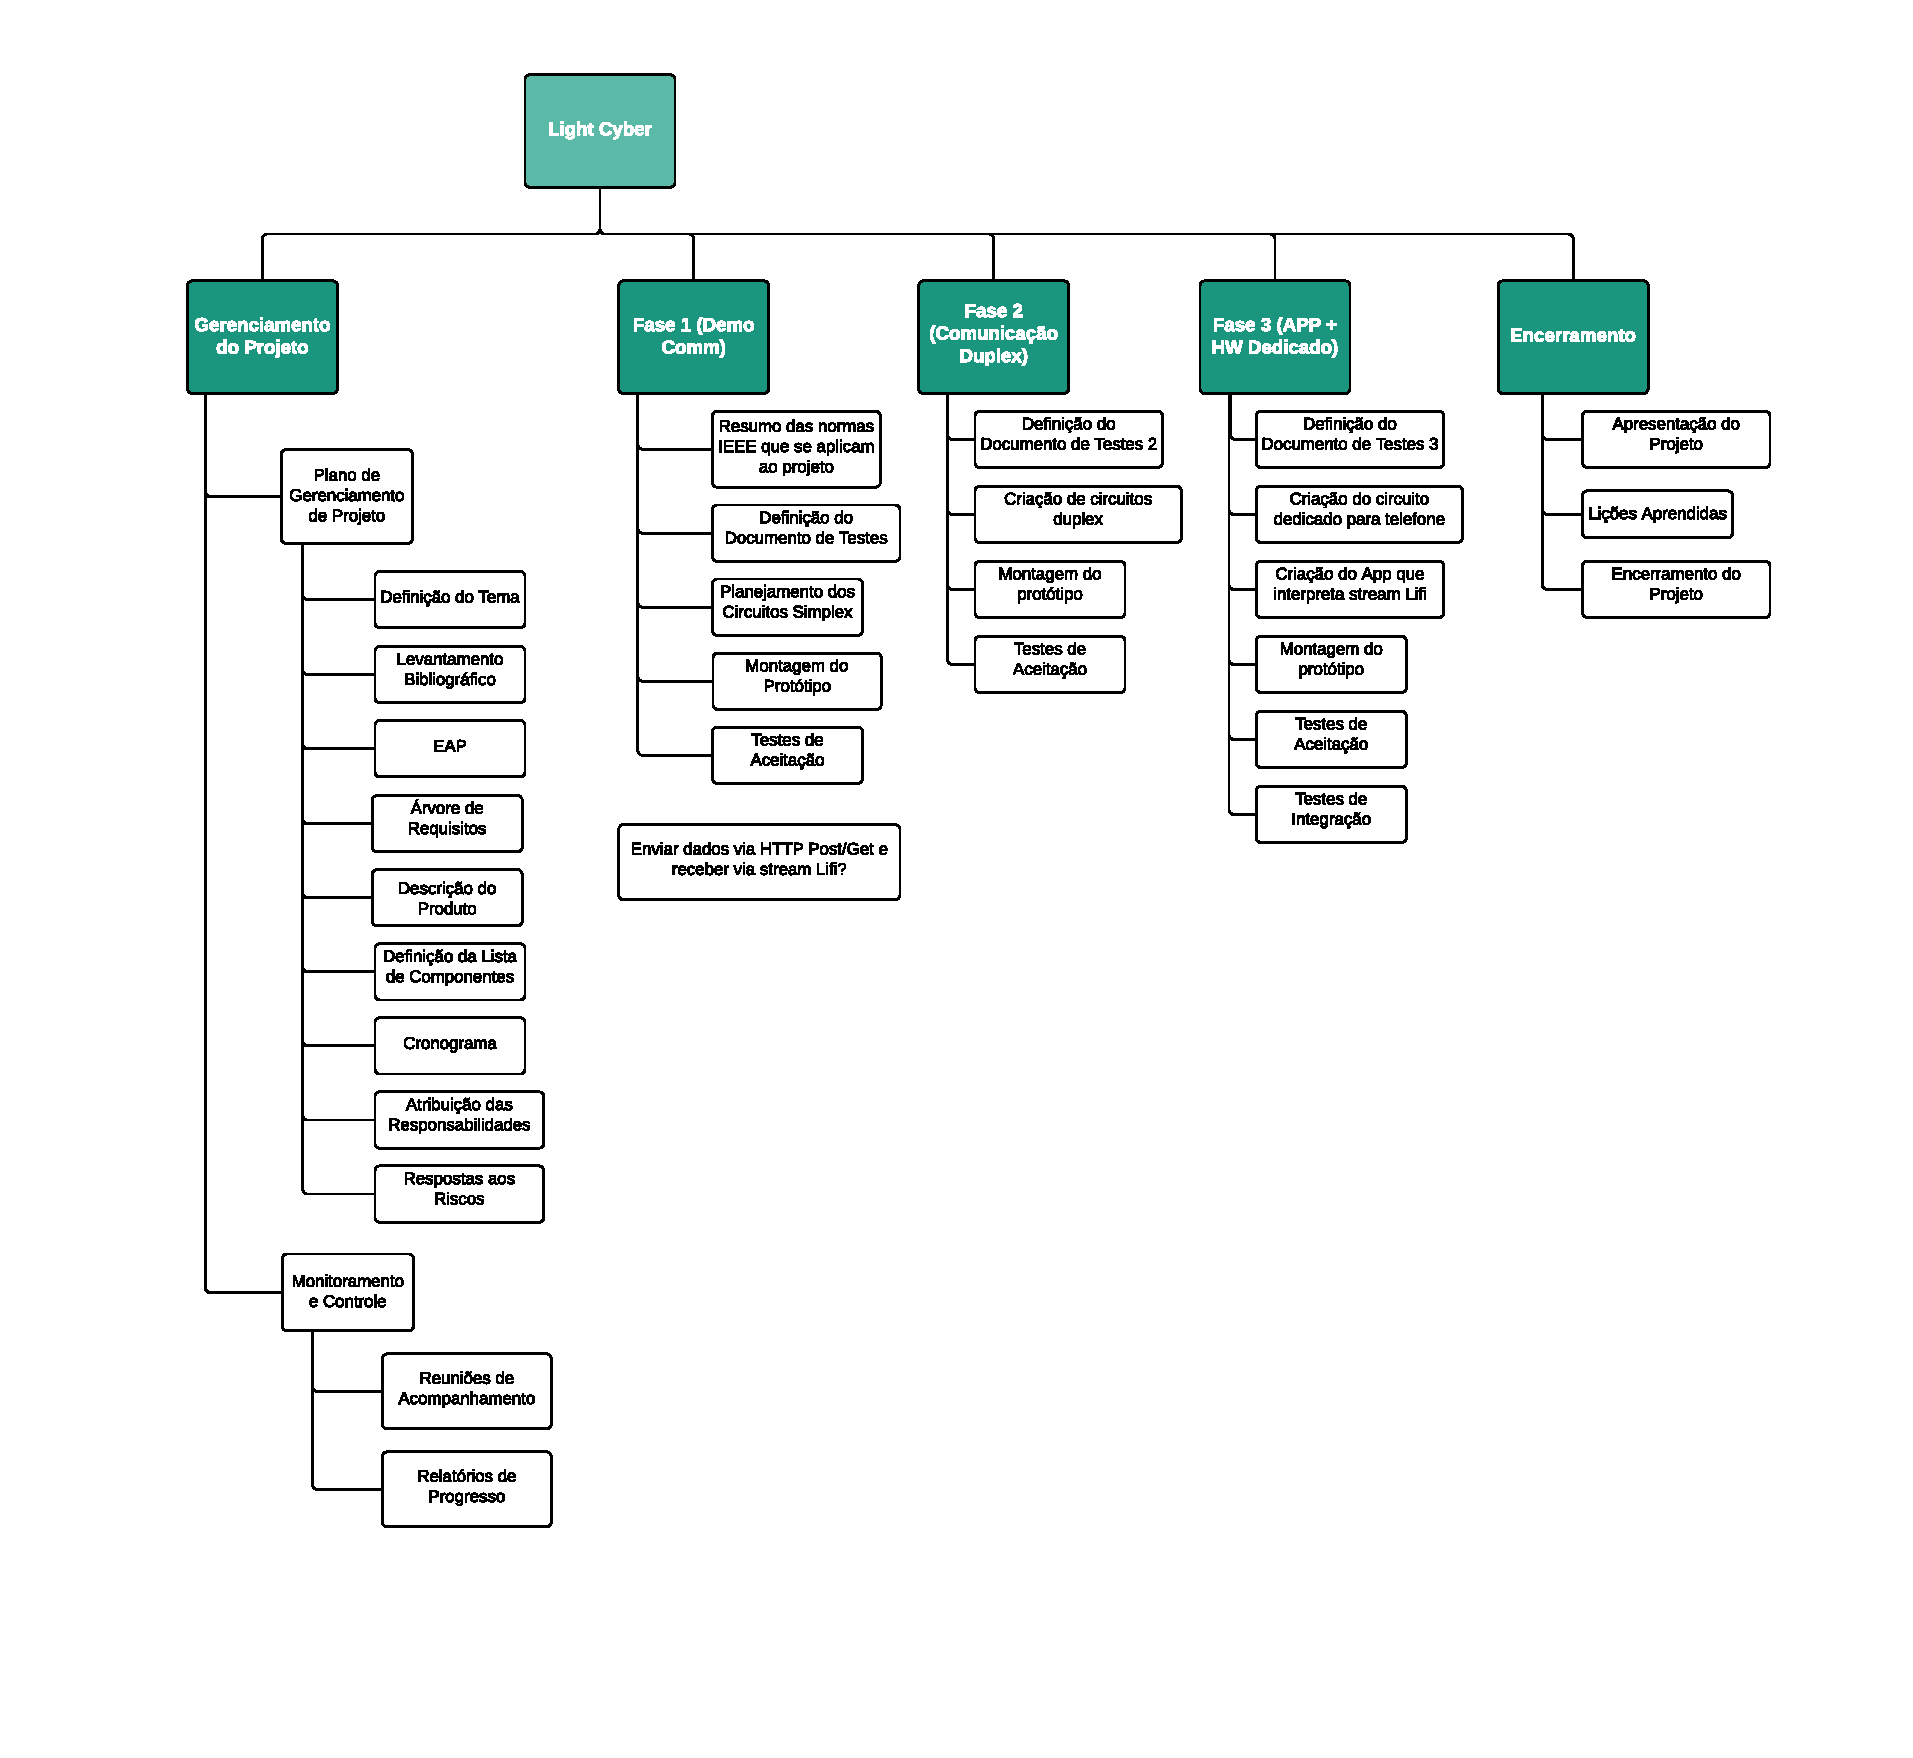
\includegraphics[width=1.0\textwidth, trim={1cm 1cm 1cm 1cm}, clip]{EAP.pdf}}
	\end{figure}
	
	% ---
	\subsection{Cronograma}\label{subsec-cronograma}
	% ---
	
	O cronograma do projeto foi planejado a partir dos pacotes de trabalho definidos na Estrutura Analítica de Projeto. Os participantes então fizeram reuniões para estimar o tempo, com a aplicação dessas estimativas a um calendário, considerando ainda as datas de entrega oficiais da disciplina. Com todas as estimativas feitas, o projeto tem a primeira e segunda fase com duração até o fim de Julho, com intuito de adiantar tanto a documentação quanto a implementação, como pode-se observar no diagrama de Gantt  \autoref{fig_gantt} abaixo.
	
	\begin{figure}[h!]
		\caption{\label{fig_gantt} Diagrama de Gantt do projeto LiCy}
		\centering
		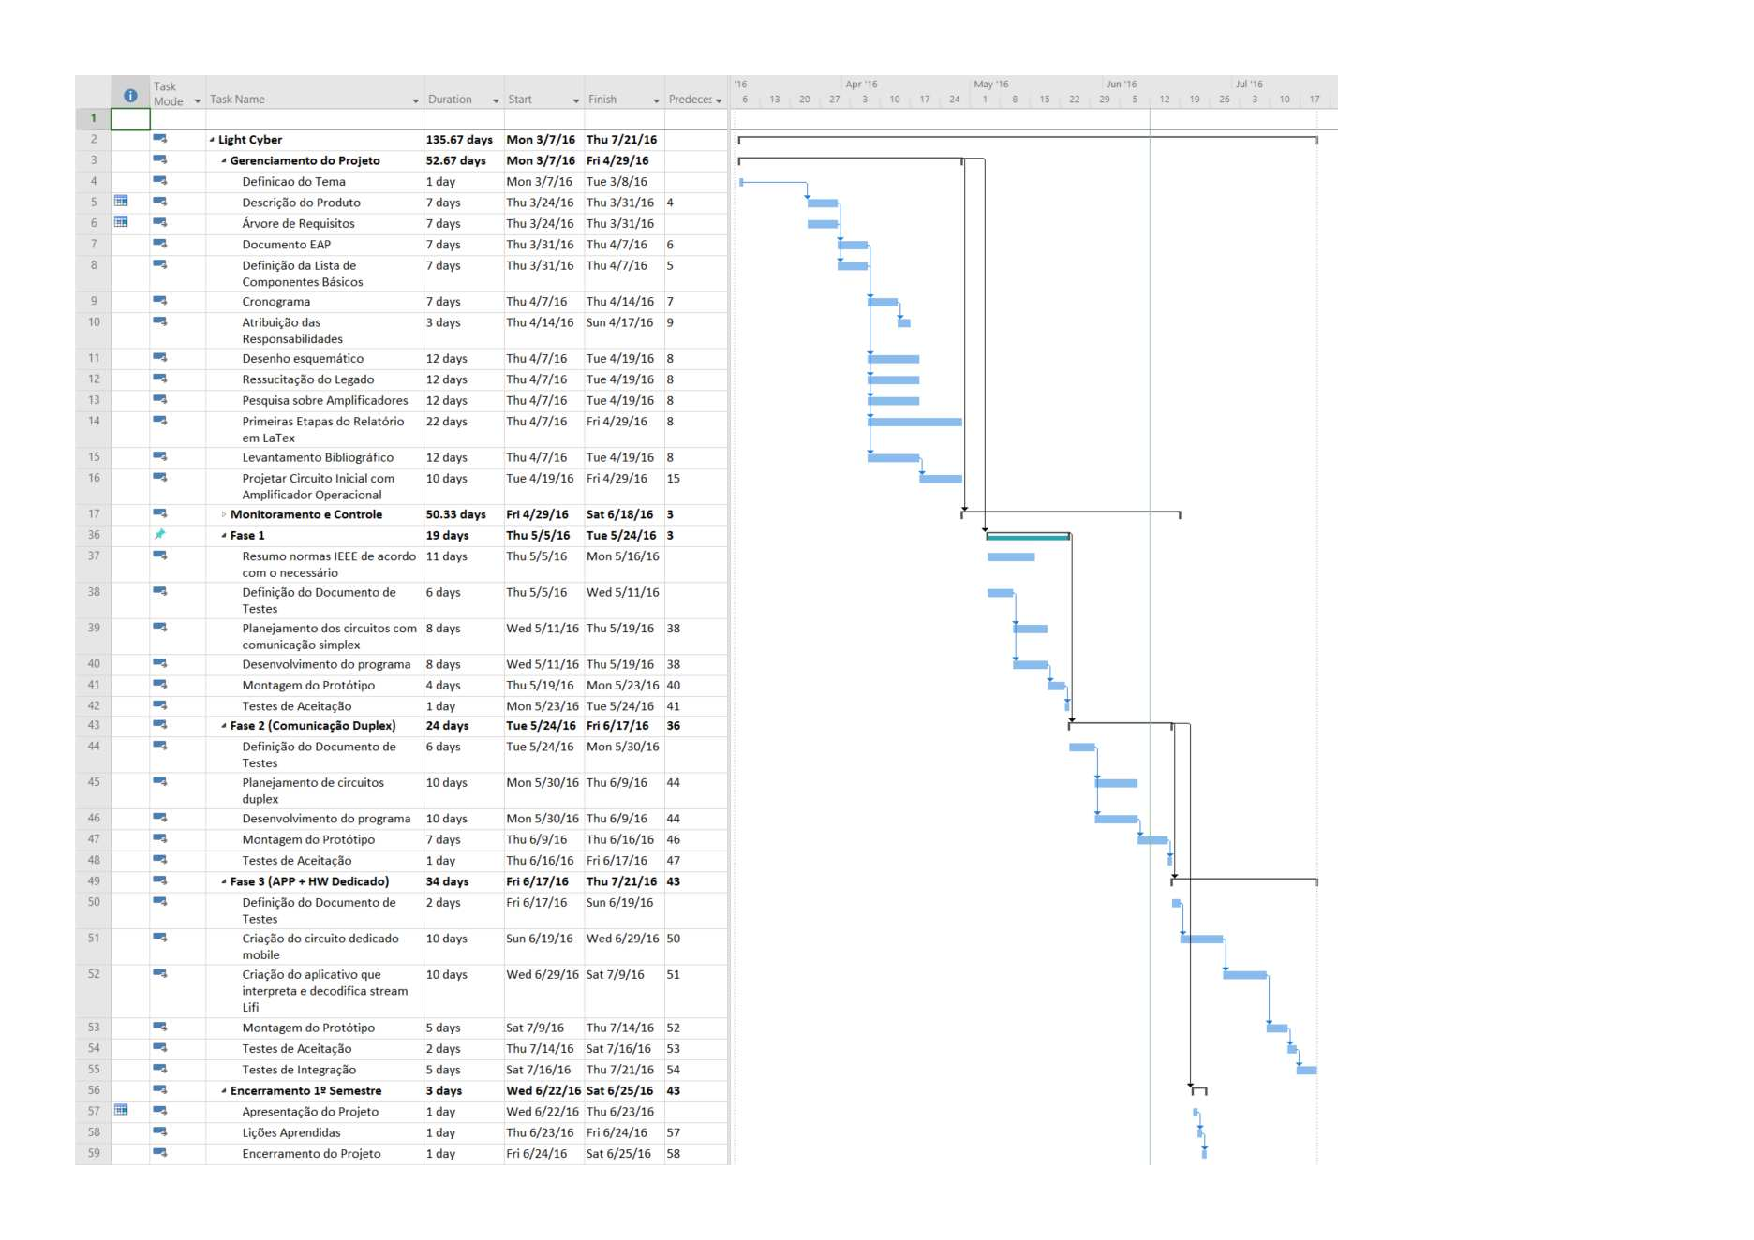
\includegraphics[width=1.0\textwidth, trim={1cm 1cm 7cm 1cm}, clip]{gantt.pdf}
	\end{figure}
	
	% ---
	\subsection{Requisitos}\label{subsec-requisitos}
	% ---
	
	Os requisitos foram divididos primeiramente em funcionais e não-funcionais. Além disso, existem outras divisões relacionadas a hardware, software, estética e módulos do sistema. Para cada requisito foi dado um peso, conforme avaliação da relevância deste requisito para este projeto, de modo que no topo da árvore haja uma soma equivalente a 1.
	
	% ---
	\subsubsection{Requisitos Funcionais}\label{subsubsec-requisitos-func}
	% ---
	\textbf{Requisitos de hardware:} é importante observar que estes dividem-se entre a lamparina, que serve de ponto de acesso, e o módulo de celular, com pesos iguais entre os dois, já que a comunicação é bilateral e ambos têm importância equivalente. Há requisitos em comum entre esses subsistemas:
	\begin{itemize}  
		\item Estar de acordo com a norma IEEE 802.15.7, que tem o peso mais alto, já que compreende o escopo principal deste trabalho, que é implementá-la;
		\item Utilização da FPGA e de um microcontrolador, para implementar as camadas física, MAC\footnote{ Media Access Control, ou camada de enlace.},  TCP, IP e de aplicação. As justificativas para o uso desses dois componentes segue nos próximos itens;
		\item Comunicação full-duplex um a um, diz respeito a garantir a bilateralidade da comunicação entre dois nós, com recepção e transmissão independentes nas duas partes;
		\item Utilizar LED e fotodiodo, para transmitir e receber, respectivamente, os dados modulados através da luz;
		\item Filtrar a luz ambiente, que é primordial para que a recepção seja bem sucedida, do contrário pode haver muita interferência da luz que não tenha o LED como fonte. Deve fazer com que o sistema se aproxime ao máximo de um cenário ideal, onde há apenas um LED e um fotodiodo num ambiente escuro.
	\end{itemize}
	
	A lamparina possui requisitos de hardware próprios, incluindo funcionar como Access Point, ou seja, fornecer acesso a uma fonte de dados, que pode ser uma rede local, um computador, a internet, entre outros. Outro requisito importante e complementar a este, é a conexão desse módulo a alguma dessas fontes através de uma interface Ethernet.
	
	Já o módulo de celular tem como requisitos de hardware exclusivos o consumo de energia através de uma bateria e a conexão ao celular através da interface USB.	
	
	\textbf{Requisitos de software:} dividem-se entre a lamparina, o módulo de celular e o aplicativo, utilizado para receber e enviar dados para este módulo. Existem requisitos que são complementares às funções de hardware, porém correspondentes às soluções de software adotadas, como a implementação da norma IEEE 802.15.7 e a comunicação full-duplex um a um. Além destes, existem os requisitos de software comuns tanto à lamparina, ou Access Point Li-Fi, como ao módulo de telefone:
	
	\begin{itemize}  
		\item Lidar com luz ambiente, ou seja, minimizar a interferência causada por ela, e mitigar o efeito de erros, corrigindo ou descartando pacotes que os contenham;
		\item Transmissão de dados pelo módulo de celular e recepção pela lamparina, representam o mesmo fluxo de dados mas de dois lados da comunicação;
		\item Transmissão de dados e multimídia pela lamparina e recepção destes pelo módulo de celular;
	\end{itemize}
	
	O módulo de celular possui um requisito de software exclusivo, que é a utilização de um protocolo conhecido para se comunicar com o celular via USB. Do outro lado, o lamparina deve se conectar à internet e lidar com os pacotes que chegarem desta rede. 
	
	Além desses requisitos, existem também aqueles referentes ao aplicativo de celular, que deve decodificar os dados recebidos via USB, deve ser desenvolvido a fim de funcionar no sistema operacional Android e deve exibir vídeos, imagens ou websites.

	\begin{figure}[h!]
		\caption{\label{fig_req1_1} Requisitos Funcionais de Hardware}
		\centering
		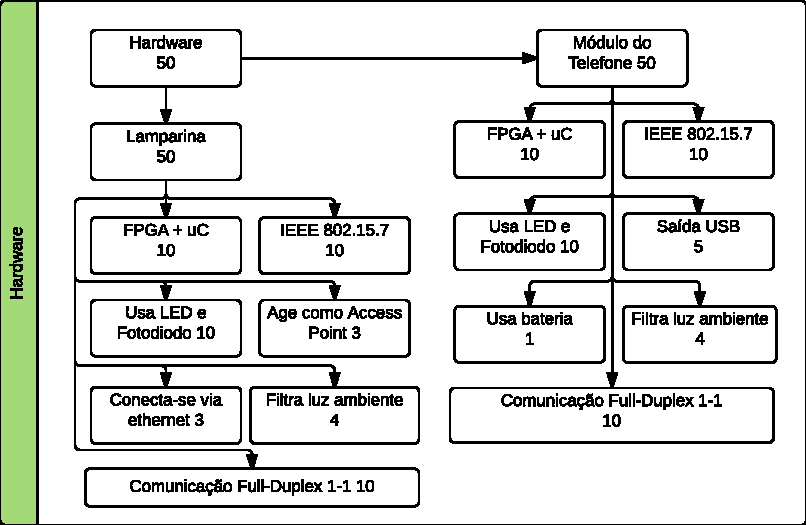
\includegraphics[width=0.8\textwidth]{ReqTree1_1.pdf}
	\end{figure}

	\begin{figure}[h!]
		\caption{\label{fig_req1_2} Requisitos Funcionais de Software}
		\centering
		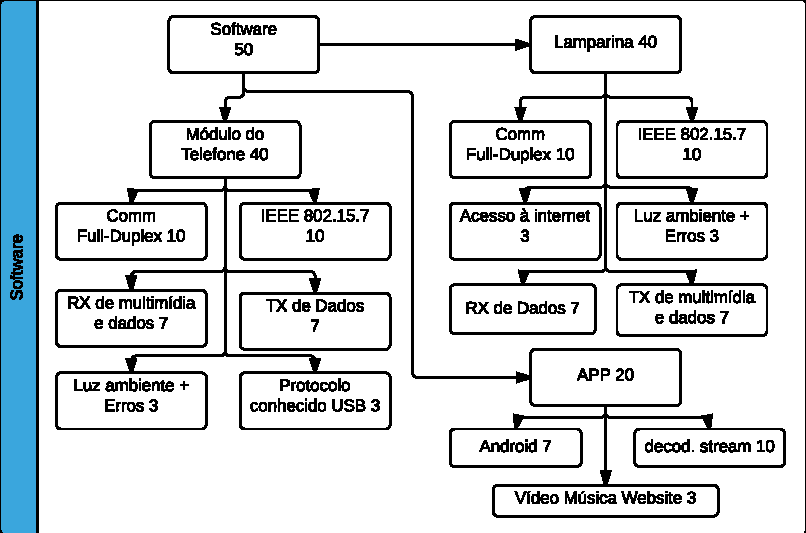
\includegraphics[width=0.8\textwidth]{ReqTree1_2.pdf}
	\end{figure}
	
	\subsubsection{Requisitos Não-Funcionais}\label{subsubsec-requisitos-nfunc}
	\textbf{Transmissão de dados:} Deve-se principalmente manter a velocidade da banda conforme a especificação da norma IEEE 802.15.7 para cada camada PHY correspondente. É também primordial garantir a confiabilidade na comunicação, ou seja, garantir que os bits recebidos estão corretos e quando possível e necessário, corrigi-los, com as limitações que serão discutidas posteriormente no que diz respeito à norma (ver módulos de codificação e decodificação). Além disso, há um requisito de segurança, que equivale a evitar a possibilidade de vazamento de dados para terceiros, ou até a intromissão de mensagens indesejadas na comunicação.
	\textbf{Modulação de luz:} O requisito mais importante é garantir o funcionamento do sistema a uma distância de até 1 metro, considerando uma aplicação residencial do produto. Secundariamente, há o requisito de manter um baixo consumo de energia, que apesar de fundamental em produtos de tecnologia da informação, foge do escopo deste estudo.
	
	\begin{figure}[h!]
		\caption{\label{fig_req2} Requisitos Não Funcionais}
		\centering		%  trim={<left> <lower> <right> <upper>} 
		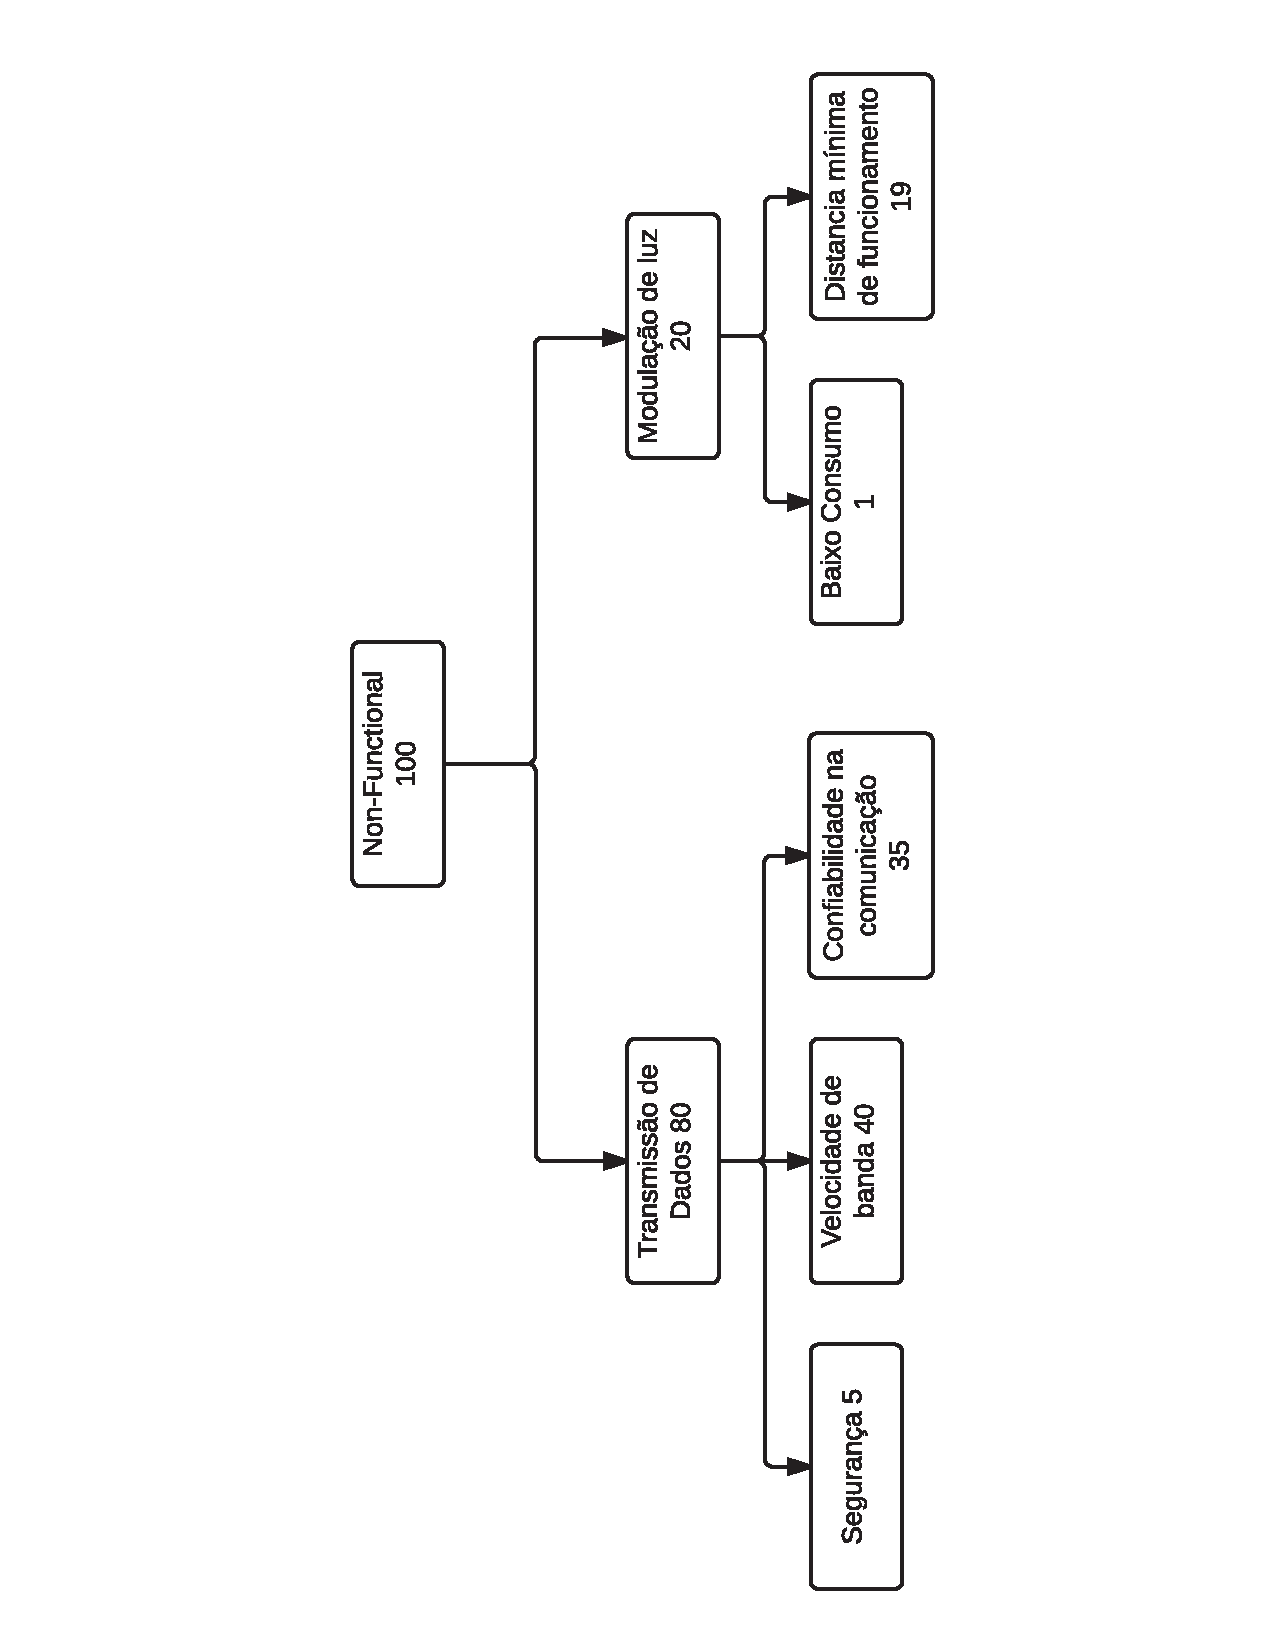
\includegraphics[width=0.9\textwidth, trim={1cm 5.5cm 1cm 6cm}, clip]{ReqTree2.pdf}
	\end{figure}
	
	\begin{figure}[h!]
		\caption{\label{fig_req3} Outros Requisitos}
		\centering
		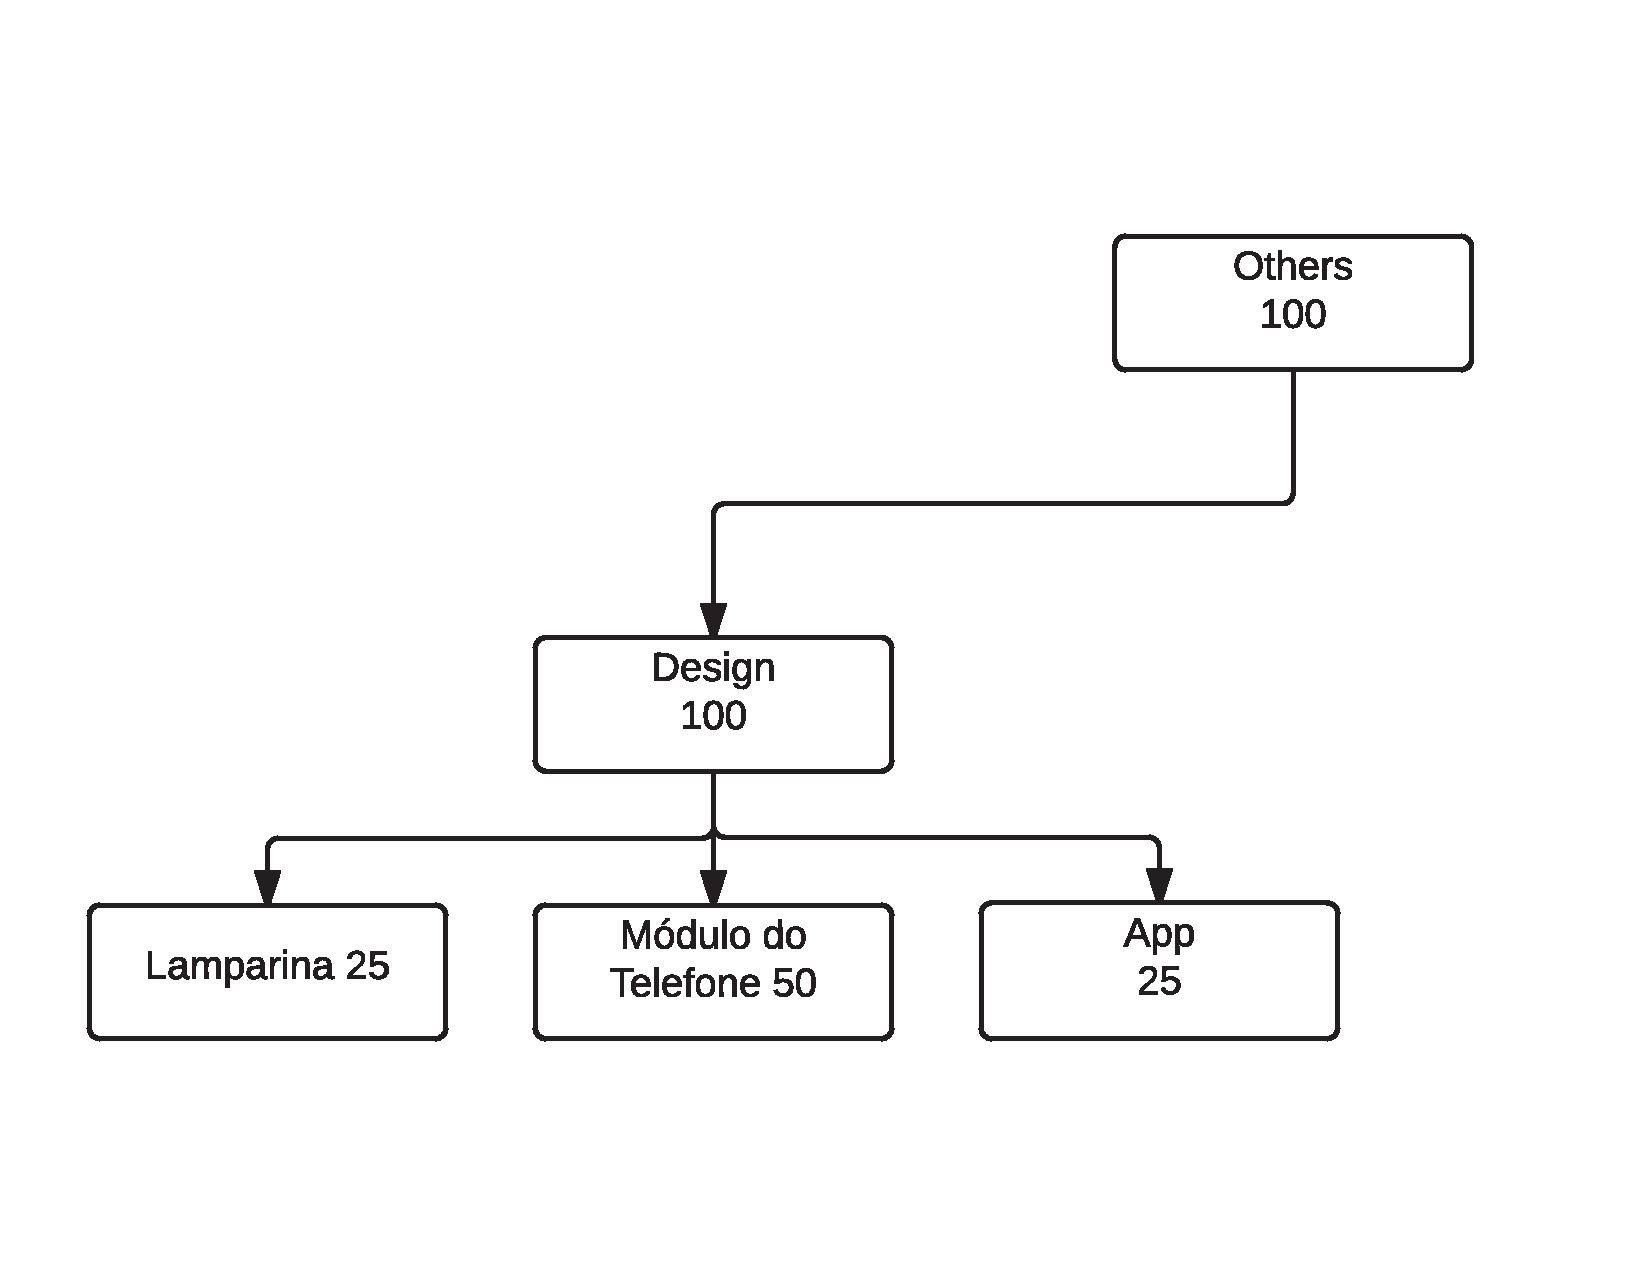
\includegraphics[width=0.7\textwidth, trim={1cm 4cm 3cm 4cm}, clip]{ReqTree3.pdf}
	\end{figure}
	
	% ---
	\section{Norma IEEE 802.15.7}\label{sec-norma}
	% ---
	
	A norma 802.15.7 estabelece um padrão para comunicação via luz, no que se diz respeito à definição de topologias de rede, codificação da informação, divisão das camadas da arquitetura do sistema de comunicação, ordem e conteúdo de cabeçalhos para cada camada e definições sobre a segurança do \textit{link}. A arquitetura de um sistema LiFi completo está definida na \autoref{fig_architecture}.
	
	\begin{figure}[htb]
		\caption{\label{fig_architecture} Arquitetura de dispositivos VPAN}
		\centering
		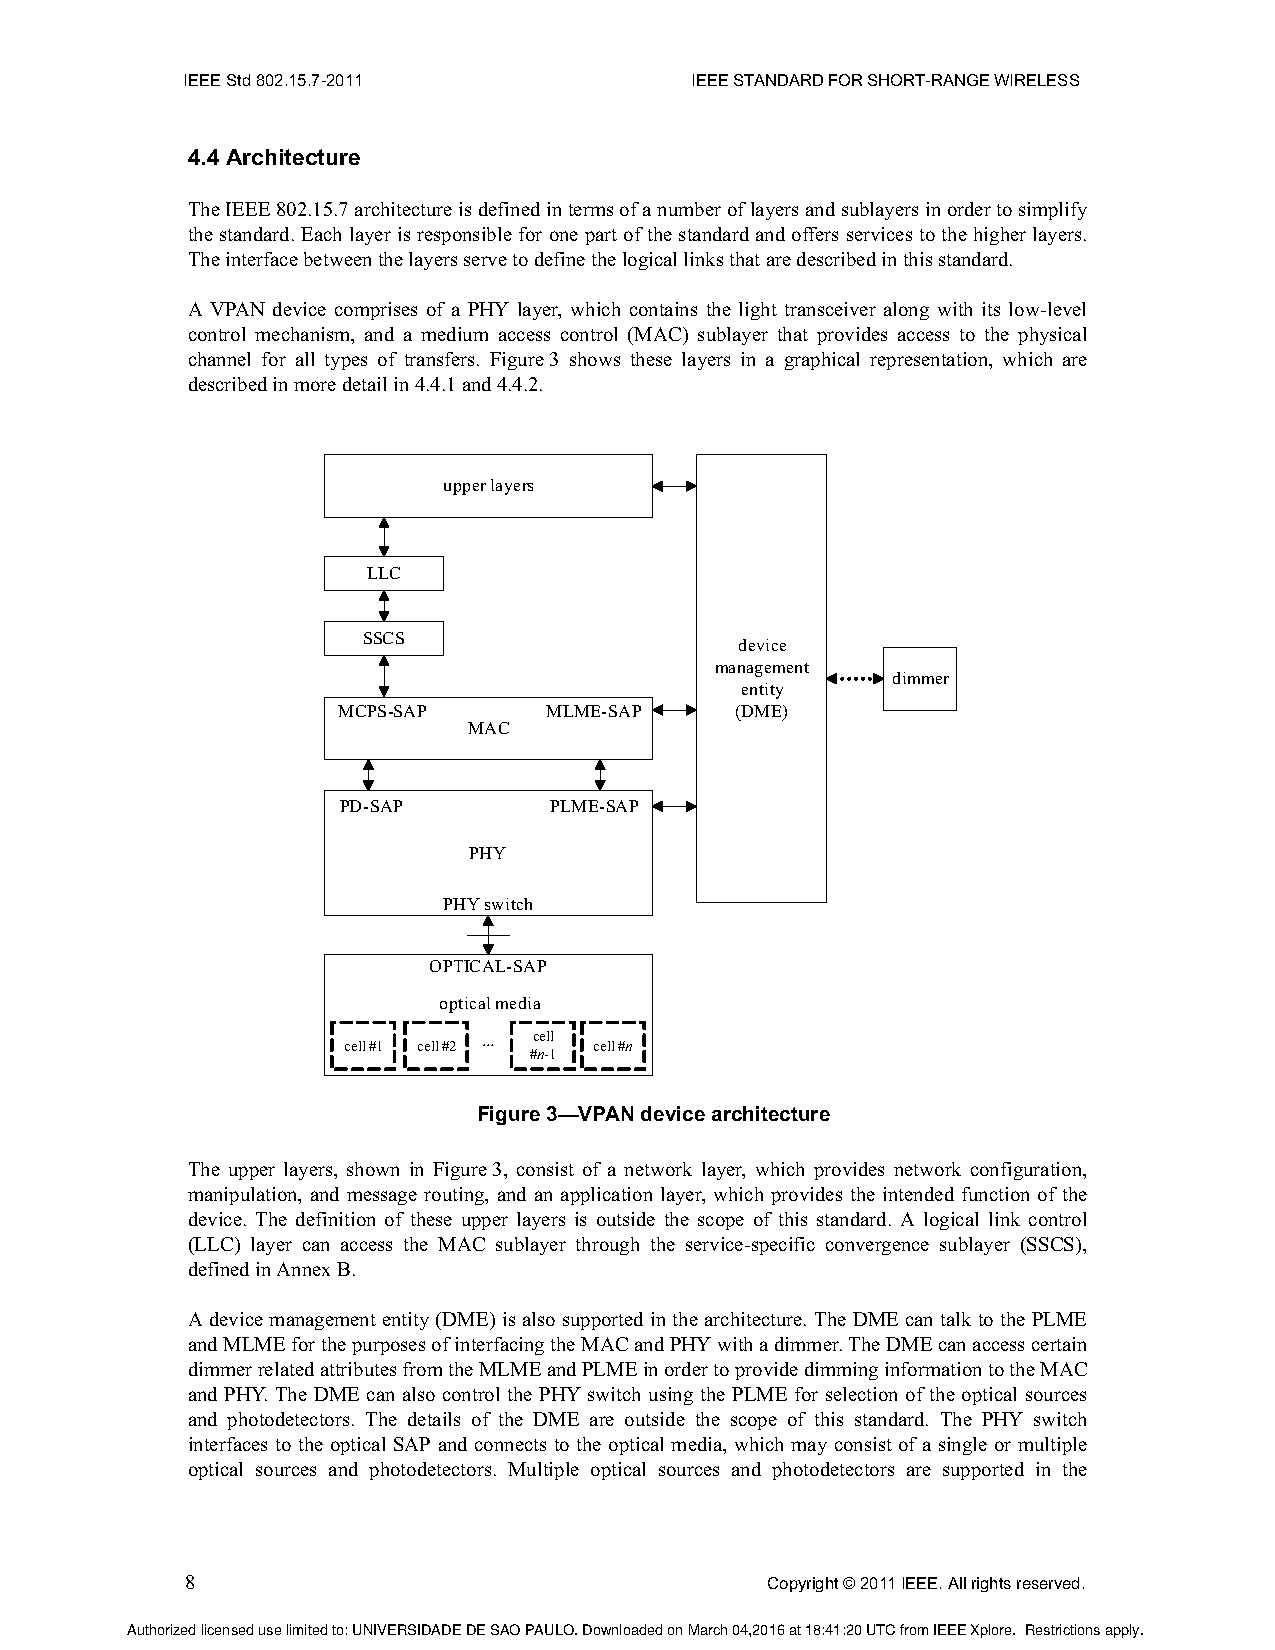
\includegraphics[width=0.5\textheight,trim={5.5cm 9.6cm 5.3cm 7cm}, clip]{pag31.pdf}
		\legend{Fonte: IEEE 802.15.7}
	\end{figure}
	
	O trabalho focará no estudo e implementação das camadas PHY e MAC.
	
%	\begin{figure}[htb]
%		\caption{\label{fig_transmission_simple_blocs} Diagrama de blocos simplificado da transmissão da camada PHY I}
%		\centering
%		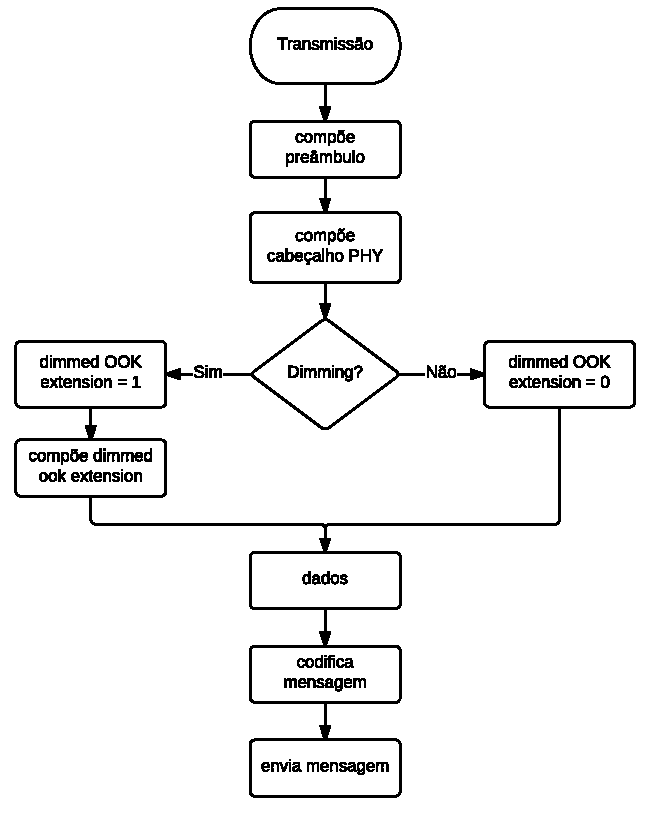
\includegraphics[width=0.4\textheight]{transmissao-blocos-simplificado.pdf}
%	\end{figure}

	\subsection{Transmissão}
	
	Nessa seção será discorrido o processo de transmissão de dados via luz, levando em conta códigos cíclicos de correção de erro, redução de erros em burst e protocolos RLL, especificados pela norma IEEE. Para realizar a transmissão, é necessário passar pelas etapas do diagrama abaixo:
		
		\begin{figure}[htb]
			\caption{\label{fig_transmission_phy1} Diagrama de blocos da codificação da mensagem}
			\centering
			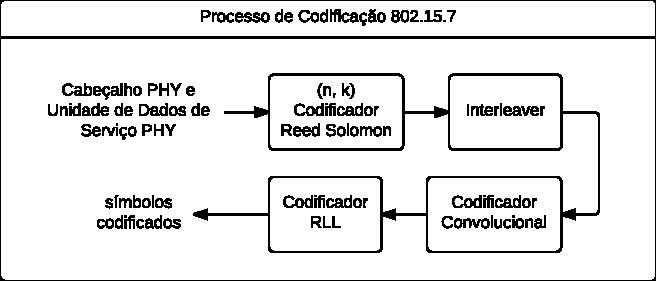
\includegraphics[width=0.6\textheight]{PHY1-transmission.pdf}
			\legend{Fonte: @todo figura 126}
		\end{figure}
		
	Para que os dados transmitidos sejam corretamente recebidos, a norma estabelece algumas regras para codificação da mensagem, a fim de garantir recuperação de erros, redução de erros em burst, maior facilidade na sincronia do clock, entre outros detalhes. A \autoref{fig_transmission_phy1} ilustra os passos necessários para compor a mensagem antes de sua transmissão. Esses passos estarão detalhados nas seções a seguir.
	
	\subsubsection{Codificação Reed Solomon}
	
	Com intuito de adicionar redundância de informação na mensagem, a norma estabelece um mecanismo de correção de erros antecipada (FEC). Mais especificamente, o código de Reed Solomon. 
	
	Os códigos Reed Solomon são compostos por símbolos de mais de um bit. O número de erros é considerado como sendo o total de símbolos com pelo menos um bit com erro. Isso o torna efetivo para corrigir erros em rajadas, já que uma sequência de bits errados dentro de um mesmo símbolo é considerada como apenas um erro. 
	
	Os principais parâmetros de um código Reed Solomon são (n, k), onde n é o número de símbolos de um bloco de código e k é o tamanho da mensagem em número de símbolos. Portanto, o bloco terá n - k símbolos de paridade, usualmente designados como 2t, sendo que a capacidade de correção é de até t símbolos.
	
	Galois Fields
	
	A codificação e decodificação de Reed Solomon usam em seus algoritmos operações aritméticas de multiplicação e adição de campos finitos. A norma 802.15.7 define que para a camada PHY 1, usa-se Galois Fields 16, ou na notação corrente na literatura: GF(16). Um campo de Galois é um conjunto de 2m - 1 elementos, cada qual representado por um polinômio de grau m - 1, com coeficientes binários. Em suma, um elemento de GF(16) pode ser representado a partir de símbolos de 4 bits, totalizando 16 elementos de 0000 a 1111. 
	
	Tabela de GF(16)
	
	A adição e subtração de dois campos de Galois é dada pela soma ou subtração dos coeficientes de dois polinômios. Além disso as operações são feitas bit a bit, sem que haja bits de "vai um" para coeficientes subsequentes. Caso os dois coeficientes tenham o mesmo valor, que pode ser 1 ou 0, o resultado da sua soma ou subtração deve ser 0. Caso contrário, a soma equivale a 1, de maneira que essa operação é perfeitamente representável pela função lógica de OU exclusivo, para ambas adição e subtração.
	
	Os campos de Galois são definidos com base no gerador polinomial de campos, que é um polinômio irredutível, de grau m. Para GF(16) existem duas possíveis opções:
	
	opções de gerador
	
	A norma IEEE 802.7.15 não especifica qual gerador polinomial deve ser usado, portanto neste estudo foi usada a opção 1. O processo de geração neste caso resulta nos seguintes elementos finitos:
	 
	 tabela de elementos
	 
	A multiplicação entre dois campos de Galois ocorre, em termos de aritmética comum, pela multiplicação de dois polinômios, seguida da divisão pelo gerador polinomial. Já a divisão  de campos finitos pode ser feita através da operação de inversão do divisor e multiplicação desse resultado pelo dividendo, seguindo os passos indicados anteriormente para a multiplicação. 
	 
	 Codificação 
	 
	Para gerar um código de Reed Solomon a partir dos campos finitos, é necessário um polinômio gerador de código. Este polinômio possui 2t fatores, de maneira que o grau do polinômio representado por C(x) (bloco codificado, com grau n) seja a soma do grau de M(X) (a própria mensagem dentro do bloco codificado, com grau k) e G(X) (polinômio codificador, com grau 2t = n - k). O polinômio gerador de código deve ter a seguinte forma:
	 
	 polinômio gerador genérico
	 
	As raízes são escolhidas como campos finitos de Galois consecutivos. Para esse estudo, usaram-se como raízes os elementos consecutivos de alpha0 a alpha7. Por exemplo, para um código (15, 7), usado posteriormente neste projeto:
	 
	cálculo do polinômio gerador 15,7
	 
	polinômio 15,7
	 
	Neste caso, a mensagem M(x) é codificada da seguinte maneira:
	 
	M(x) * x elevado a n-k dividido por G(x)
	 *por a fórmula*
	 
	Desta forma, são produzidos um quociente q(x) e um resto r(x). Por manipulação algébrica, temos que o bloco codificado pode ser representado da seguinte forma:
	 
	M(x)x x(n-k) + r(x) = g(x) x q(x)
	 
	Portanto o bloco codificado C(x) é composto por M(x) deslocada, somada a r(x), na prática equivalendo às seguintes code words (por referência explicando o que é cw):
	 
	 *desenho do bloco M(x) + r(x)*
	 
	Finalmente, o codificador de Reed Solomon (15, 7) em hardware equivale a:
	 
	 
	Decodificação:
	
	Cálculo das síndromes:
	
	As síndromes são calculadas através da mensagem recebida e dos símbolos de paridade. O objeto desse cálculo é identificar num primeiro momento a presença de erros no que foi recebido em relação ao que foi transmitido. Utilizaremos aqui a notação de R(x) para o bloco recebido e E(x) para os possíveis erros. Portanto:
	
	R(x) = C(x) + E(x)
	
	Caso a mensagem recebida não tenha erros, teremos E(x) formado por 15 símbolos de 0000 no caso de Reed Solomon (15, 7). Se pelo menos um símbolo de E(x) possuir pelo menos um bit diferente de 0, configura-se um erro, e o cálculo das síndromes deverá apontá-lo. Caso o número de símbolos com erro exceda t, ou 4 símbolos para um código (15, 7), o erro será identificado nas síndromes, porém não será possível corrigi-lo posteriormente.
	
	No caso de Reed Solomon, as síndromes podem se definir da seguinte maneira:
	
	Si = Qi(x)*(x + alphai) + R(x)
	
	No caso específico em que x é alphai, temos que o primeiro termo da soma é nulo, já que x + alphai = 0000. Portanto:
	
	Si = R(alphai)
	
	E haverá um total de 2t síndromes, uma para cada raiz do polinômio codificador G(x). Considerando que existem v símbolos com erros, com v <= t, teremos:
	
	E(x) = V1*xL1 + ... + Vv*x Lv
	
	Com Vi representando os valores do erro, e Li indicando a localização desses erros. Portanto, para cada Síndrome Si:
	
	Si(alphai) = V1*X1i + V2*X2i + ... Vv*Xvi
	
	Os valores de Xi são usualmente designados para representar os localizadores de erro. Observe que os índices numéricos não necessariamente indicam o coeficiente do polinômio.
	
	Uma possível representação para o cálculo da síndrome, em hardware, seria:
	
	Localização dos erros:
	
	O polinômio localizador de erros é construído com auxílio dos localizadores de erro, denotados por X1 a Xv.
	
	sigma(x) = (1 + x*X1)(1 + x*X2)...(1 + x*Xv)
	sigma(x) =  1 + sigma1*x1 + ... + sigmav-1*xv-1 + sigmav*xv
	
	Dessa forma teremos os inversos de X1 a Xv como raízes deste polinômio, sendo que cada uma dessas raízes torna sigma(x) igual a zero. 
	
	sigma(Xi -1) = sigmav*xi-v + ... + sigma1*xi-1 + 1 = 0
	
	Multiplicando essa igualdade por Vi*Xi i+v, temos:
	
	...
	
	Para diferentes valores de j, temos:
	
	...
	
	Dessa forma, pode-se construir a seguinte matriz com um sistema de equações:
	
	*Tabela*
	
	
	Resolvendo esse sistema, encontram-se os coeficientes do polinômio localizador de erros. Essa resolução pode se feita de mais de uma forma, porém neste estudo aborda-se o método de Berlekamp. Este algoritmo resolve o sistema por meio de aproximações sucessivas do polinômio localizador, iniciando com sigma(x) = 1.
	
	Uma vez calculados os coeficientes do polinômio localizador, 
	deve-se descobrir o valor de suas raízes. Como apontado anteriormente, o inverso destas aponta a localização dos erros. Esses valores são encontrados através do método de busca de Chien, que utiliza tentativa e erro, com todos os possíveis valores das raízes.
	
	Valores dos erros:
	
	Existem diversas maneiras de encontrar os valores dos erros. O método abordado aqui - o algoritmo de Forney - utiliza o polinômio avaliador de erros, definido como:
	
	Omega(x) = Omegav-1*xv-1 + ... + Omega1x + Omega0

	Os valores dos erros são dados por sua vez por:
	
	Vi = Xi 1-b Omega(Xi -1) dividido por Sigma'(Xi -1)
	
	Sendo Omega'(Xj -1) a derivada de Sigma(x), e b o índice do primeiro Alpha usado no polinômio codificador, que neste caso será 0.
	
	Síntese
	
	Um decodificador de Reed Solomon pode ser dividido funcionalmente nos seguintes módulos:
	
	Diagrama de decodificador
	
	
	Estratégia
	
	O primeiro passo para aproximar os algoritmos de uma solução em hardware foi procurar níveis de abstração intermediários. O nível encontrado foi a programação em alto nível, reduzindo módulos como multiplicadores e somadores a funções. Uma das vantagens deste método foi a geração de saídas esperadas para cada módulo funcional, incluindo o bloco de saída final, corrigido ou a ser descartado. Esses dados foram fundamentais para a depuração e correções em hardware. Entretanto, uma das limitações deste método era a de que a linguagem de programação pertence a um paradigma diferente do da descrição de hardware, o que envolveu o uso de máquinas de estado no lugar de loops, por exemplo.  
	
	
	\cite{nasa-rs1}

	\begin{figure}[htb]
		\caption{\label{fig_reed_solomon_message} Diagrama de blocos da codificação da mensagem}
		\centering
		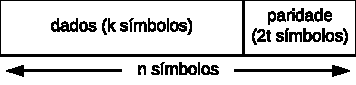
\includegraphics[width=0.5\textheight]{reed_solomon_message.pdf}
	\end{figure}	
	
	\subsubsection{Padding}
	
	Esse processo se aplica a mensagens curtas e consiste em preencher espaços vazios com zeros.
	
	\subsubsection{Interleaver}
	
	O processo de entrelaçamento é utilizado para aprimorar a performance de mecanismos de correção de erros antecipados. Ele se baseia no fato de que canais de comunicação não são estocásticos, então erros ocorrem em sequência e não independentemente. 
	
	O entrelaçamento serve para distribuir os erros em sequência, facilitando o processo de recuperação de erros, pois os erros serão distribuídos em múltiplas palavras de código. 
	
	Para melhor demonstrar a aplicação do entrelaçador, serão exemplificadas várias situações utilizado um sistema de recuperação de erros em um canal com ruídos (que costumam ser \textit{bit-flip}). Na primeira, não é aplicado o entrelaçamento e a mensagem é recuperável com redundância.

	\begin{verbatim}
	   Burst = 2, Redundância = 3, Sem entrelaçamento
	   Mensagem inicial:                             abcdefg
	   Mensagem com redundância:                     aaabbbcccdddeeefffggg
	   Transmissão com erros em burst:               aaabbbc__dddeeefffggg
	   Mensagem recuperada:                          abcdefg
	\end{verbatim}

	Mesmo após dois caracteres perdidos em sequência, foi possível recuperar as perdas do canal. Isso ocorreu pois o burst do erro foi menor que sua capacidade de recuperação. Na situação a seguir, novamente sem entrelaçamento, a mensagem não é recuperável com redundância.
	
	\begin{verbatim}
	   Burst = 4, Redundância = 3, Sem entrelaçamento
	   Mensagem inicial:                             abcdefg
	   Mensagem com redundância:                     aaabbbcccdddeeefffggg
	   Transmissão com erros em burst:               aaabbbcc____eeefffggg
	   Mensagem recuperada:                          abc_efg
	\end{verbatim}
	
	Mesmo com a redundância aplicada, a informação \textit{d} foi perdida devido à erros em burst. Aplicando entrelaçamento, a mesma mensagem pode ser recuperada facilmente, a seguir:
	
	\begin{verbatim}
	   Burst = 4, Redundância = 3, Com entrelaçamento
	   Mensagem inicial:                             abcdefg
	   Mensagem com redundância:                     aaabbbcccdddeeefffggg
	   Interleaving:                                 abcdefgabcdefgabcdefg
	   Transmissão com erros em sequência:           abcdefgab____gabcdefg
	   Deinterleaving:                               aaabbbc_cd_de_ef_fggg
	   Mensagem recuperada:                          abcdefg
	\end{verbatim}
	
	A mensagem recebida foi recuperada pois os erros foram distribuídos em partes diferentes da mensagem, que foi entrelaçada. Os dados resultantes puderam ser inferidos pela redundância aplicada. A norma especifica alguns parâmetros que devem ser definidos para criar o entrelaçador:
	
	\begin{verbatim}
	n: RS codeword length
	k: Number of information data symbols in a RS codeword
	q: Number of elements in the Galois field: GF(q)
	L_{frame}: Input frame size in bytes
	S_{frame}: Number of symbols at the input of the RS encoder
	S: Number of symbols from the output of the shortened RS encoder
	S_{block}: The size of the interleaver used
	D:The interleaving depth
	i: Ordered indices take the values 0, 1, …, Sblock–1
	l(i): Interleaved indices
	p: Number of zero RS symbols
	t: Ordered indices take the values 0, 1, …, p
	z(t): Locations of the bits to be punctured at the output of the 
	interleaver before transmission 
	\end{verbatim}
	
	\subsubsection{Puncture}
	
	O módulo de punção é utilizado para reduzir o overhead do padding, e é aplicado depois do interleaver.
	
	\subsubsection{Convolutional Encoder}
	
	Este módulo 
	
	\subsubsection{Codificação RLL}
	
	Para a primeira camada de implementação PHY I, será escolhida codificação RLL Manchester, que é codifica os bits 0 e 1 de acordo com a \autoref{tabela_cod_manchester}. Após 
	
	\begin{table}[ht]
		\caption{Codificação Manchester}
		\centering
		\begin{tabular}{c c}
			\hline
			bit & manchester symbol \\ \hline
			0 & 01 \\
			1 & 10 \\ \hline
		\end{tabular}
		\label{tabela_cod_manchester}
		\legend{Fonte: Tabela 103 da norma 802.15.7}
	\end{table}
	
	\subsection{Recepção}
	
	Após a codificação dos dados, é necessário realizar a decodificação deles. Para isso, deve-se reverter os processos aplicados pela seção anterior. No entanto, isso não é tão trivial, dado que vários desses módulos devem realizar correção de erro, tornando o algoritmo completamente diferente. As etapas de decodificação dos dados estão esquematizadas abaixo:

	\begin{figure}[htb]
		\caption{\label{fig_transmission_phy1} Diagrama de blocos da codificação da mensagem}
		\centering
		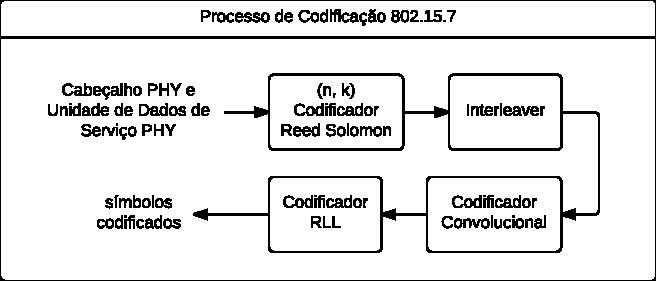
\includegraphics[width=0.6\textheight]{PHY1-transmission.pdf}
		\legend{Fonte: @todo figura 126}
	\end{figure}

	Esses passos estarão detalhados abaixo:
	
	
	\subsubsection{Decodificação RLL}
	\subsubsection{Decodificação Viterbi}
	\subsubsection{Puncture}
	\subsubsection{Deinterleaver}
	\subsubsection{Decodificação Reed Solomon}
	
	% ---
	\section{Hardware}\label{sec-hardware}
	% ---
	
	A seguir serão discorridas as implicações da implementação da norma IEEE 802.15.7 em um escopo de hardware analógico, a partir da necessidade de transmitir, receber e converter sinais digitais em analógicos, que então serão convertidos de/para oscilações luminosas.
	
	A \autoref{fig_dataflow_analog_circuits}  representa o fluxo que os dados devem fazer:
	
	\begin{figure}[htb]
		\caption{\label{fig_dataflow_analog_circuits} Diagrama de blocos da conversão digital-analógica e analógica-digital da transmissão de dados.}
		\centering
		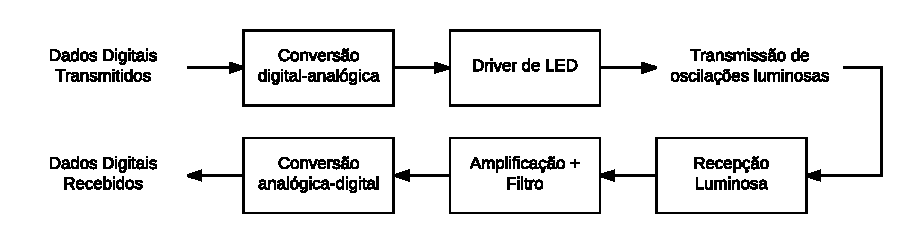
\includegraphics[width=0.6\textheight]{circuits/dataflow_analog_circuits.pdf}
		\legend{Fonte: autores.}
	\end{figure}
	
	Os dois primeiros módulos são relativos ao circuito de recepção, enquanto os três últimos são relativos ao transmissor.
	
	% ---
	\subsection{Transmissão}
	% ---
	
	O transmissor do sistema de comunicação LiCy será composto por um conversor digital-analógico e um LED de potência. Os dados serão enviados a partir da FPGA e codificados em 0 e 3.3V, representando os sinais \texttt{0} e \texttt{1} digitais. 
	
	Para cada um desses módulos deve haver um minucioso estudo sobre suas características eletro-eletrônicas, pois existem muitas restrições que devem ser levadas em conta com a frequência de operação $F_{op} = 200 kHz$, como:
	
	\begin{itemize}  
		\item Ruídos são amplificados nessa frequência;
		\item Capacitâncias e Indutâncias parasitas em todos componentes, com ênfase no LED e no transistor;
		\item Prototipação dificultada, pois a breadboard possui muita capacitância em seus contatos;
		\item Alta corrente para ligar um LED de potência.
		\item Componentes limitados pela frequência de operação.
	\end{itemize}
	
	Contornando e solucionando todas as restrições listadas acima, o circuito resultante deverá enviar sinais luminosos a uma frequência de 200kHz.

	\begin{comment}
	\texttt{Colocar desenho de FPGA enviando dados}
	
	É proposto um circuito que associa o transistor em modo emissor comum e o LED conectado no 	
	
	Para o envio de daos
	O LED escolhido deverá ter uma curva de resposta de tensão semelhante ao de um diodo. A 
	Para realizar a transmissão, deve-se realiz
	Falar sobre curva de potencia do led, e de como passar do corte para saturação (desligando e ligando) muito rápido trabalha dentro da área não linear de operação do LED (nem está marcada no datasheet). Então foi escolhida uma técnica utilizada em vários sistemas de VLC e transmissão de fibra ótica: trabalhar com um Vdc e apenas variar a tensão dentro na saturação.
	
	@todo	Precisa de mais bibliografia.
	\end{comment}
	
	\subsubsection{Conversor Digital-Analógico}
	Como o LED será de alta potência, a corrente necessária para ligá-lo corretamente é na ordem de grandeza de amperes, incompatível com a corrente fornecida pela porta de saída da FPGA. Como forma de proteger o circuito da FPGA e também chavear o LED, será utilizado um transistor de potência.
		
	O intuito é deixá-lo na configuração de fonte comum (\autoref{fig_common_source}, agindo como chave entre o circuito do LED, VCC e GND.
		
	\begin{figure}[htb]
		\caption{\label{fig_common_source} FET em modo de fonte comum.}
		\centering
		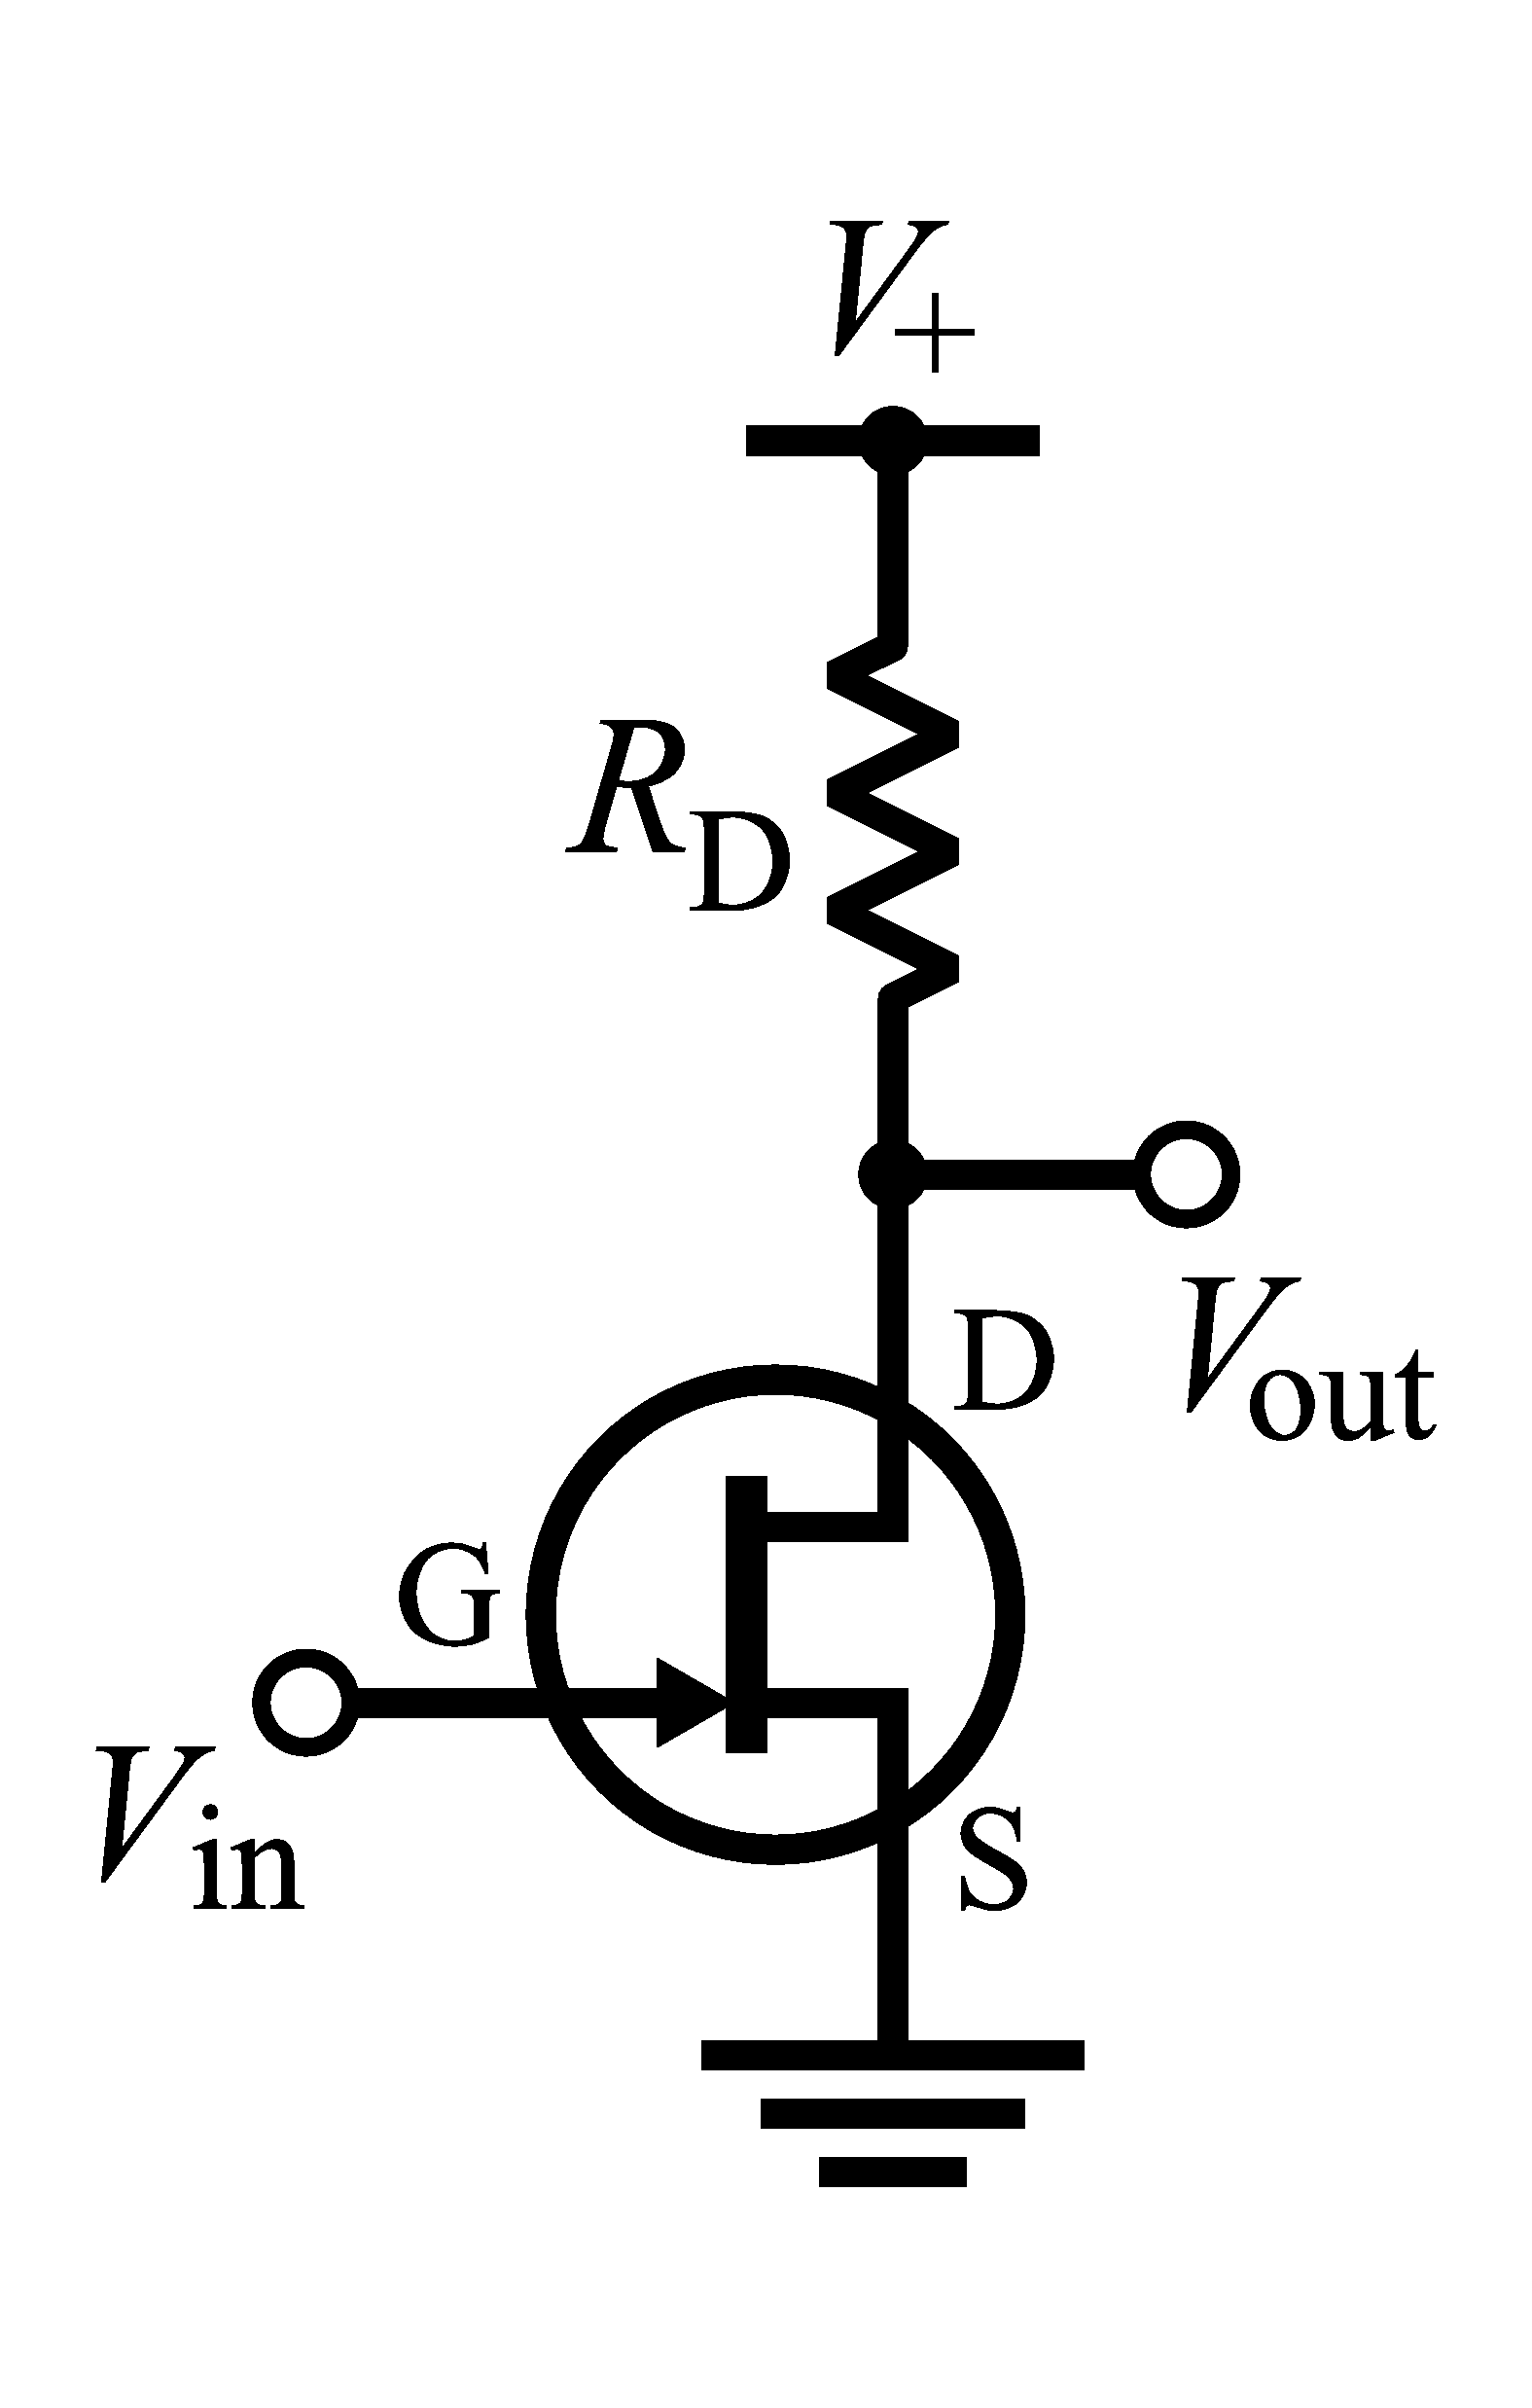
\includegraphics[width=0.2\textwidth]{circuits/common_source.pdf}
		\legend{Fonte: Wikipedia}
	\end{figure}

	% ---
	\subsubsection{LED}\label{hard-led}
	% ---
	
	De acordo com a \autoref{tab_phy1} e \autoref{tab_phy2}, para cada camada física implementada é necessário suportar uma frequência de oscilação luminosa mínima:
	
	\begin{itemize}
		\item PHY I: 400kHz
		\item PHY II: 120MHz
	\end{itemize} 
	
	O LED para a transmissão deverá então suportar essas frequências de acordo com a implementação de cada camada. Além disso, também deve realizar a transmissão de luz a distâncias de pelo menos um metro.
	
	Será então necessária a utilização de um LED de potência. É muito importante que o LED escolhido tenha resposta luminosa de acordo com o chaveamento, de forma que a tensão fornecida seja proporcional a luz emitida. Caso esse último requisito não seja atendido, será muito difícil realizar uma transferência confiável de dados.
	
	% ---
	\subsection{Recepção}
	% ---
	
	O receptor é obrigado a identificar essas variações minúsculas na luminosidade e para isso deve ser utilizado no modo fotocondutivo com uma amplificação alta (
	
	Fig. 2 shows a inverting TIA with the photodiode driven by a laser diode and operating in the photoconductive mode. A positive voltage at the cathode of the photodiode applies a reverse bias. This reverse bias increases the width of the depletion region and lowers the junction capacitance, improving the high frequency performance. The photoconductive configuration of a transimpedance photodiode amplifier is used where fast switching speed is required but high gain is not. The feedback capacitor, Cf is usually required to improve stability.
	
	)
	
	Após o estágio de recepção propriamente dito utilizando o Amplificador de Transimpedância e o fotodiodo, é realizado um estágio de amplificação com comparação, para transformar o sinal analogico recebido em uma onda quadrada. Com a sensibilidade ajustada de acordo, é possível que o sinal recebido seja muito semelhante (se não exatamente igual) ao enviado. Após esse estágio pode ser necessário realizar a retificação da onda com um outro comparador, um schmitt trigger hex inverter nesse caso.
	
	http://electronicdesign.com/analog/whats-all-transimpedance-amplifier-stuff-anyhow-part-1

	% ---
	\subsubsection{Fotoreceptor}\label{hard-photodiode}
	% ---
	
	O módulo mais crítico do receptor, que recebe oscilações luminosas e converte-as em sinais analógicos. É muito empregado em circuitos receptores de fibra óptica, CD players, televisões, câmeras e até em medidores de batimento cardíaco. Os fotoreceptores mais comuns são fototransistores ou fotodiodos, que são classificados principalmente de acordo com sua velocidade de chaveamento. 
	
	Um fototransistor é composto por um transistor de junção que responde à incidencia de luz gerando e amplificando corrente elétrica. Seu tempo de resposta é da ordem de $\mu$s. Já o fotodiodo é um diodo semicondutor que gera diferença de potencial ou mudança em sua resistência quando iluminado, com o tempo de resposta usualmente em ns.
	
	Para o projeto, é mais interessante a escolha do fotodiodo, pela sua alta velocidade de resposta, tornando a onda recebida mais fiel possível a realidade.
	
	O fotodiodo tem dois principais modos de operação com as seguintes características:
	
	\begin{table}[ht]
		\caption{Comparação entre modos de operação do fotodiodo.}
		\centering
		\begin{tabular}{c c c}
			\hline
			Modo de Operação  & Polarização & Características \\ \hline
			Fotovoltaico & não & $I_{dark}$ menor, resposta mais lenta \\
			Fotocondutivo & negativa & $I_{dark}$ maior, resposta muito rápida \\ \hline
		\end{tabular}
		\label{tab_photodiode_comp}
	\end{table}
	
	% ---
	\subsubsection{Amplificadores Operacionais}\label{hard-opamp}
	% ---
	
	Amplificadores operacionais são 
	A seguir serão exemplificados três modos de operação com amplificadores operacionais. 
	\paragraph{Passa-faixas}
	Com intuito de reduzir o ruido da luz ambiente, o circuito passa-faixas amplificador a seguir (\autoref{fig_opampdif}) foi proposto para o projeto.
	
	\begin{figure}[h!]
		\caption{\label{fig_opampdif}Circuito amplificador de diferenças.}
		\centering
		%  trim={<left> <lower> <right> <upper>} 
		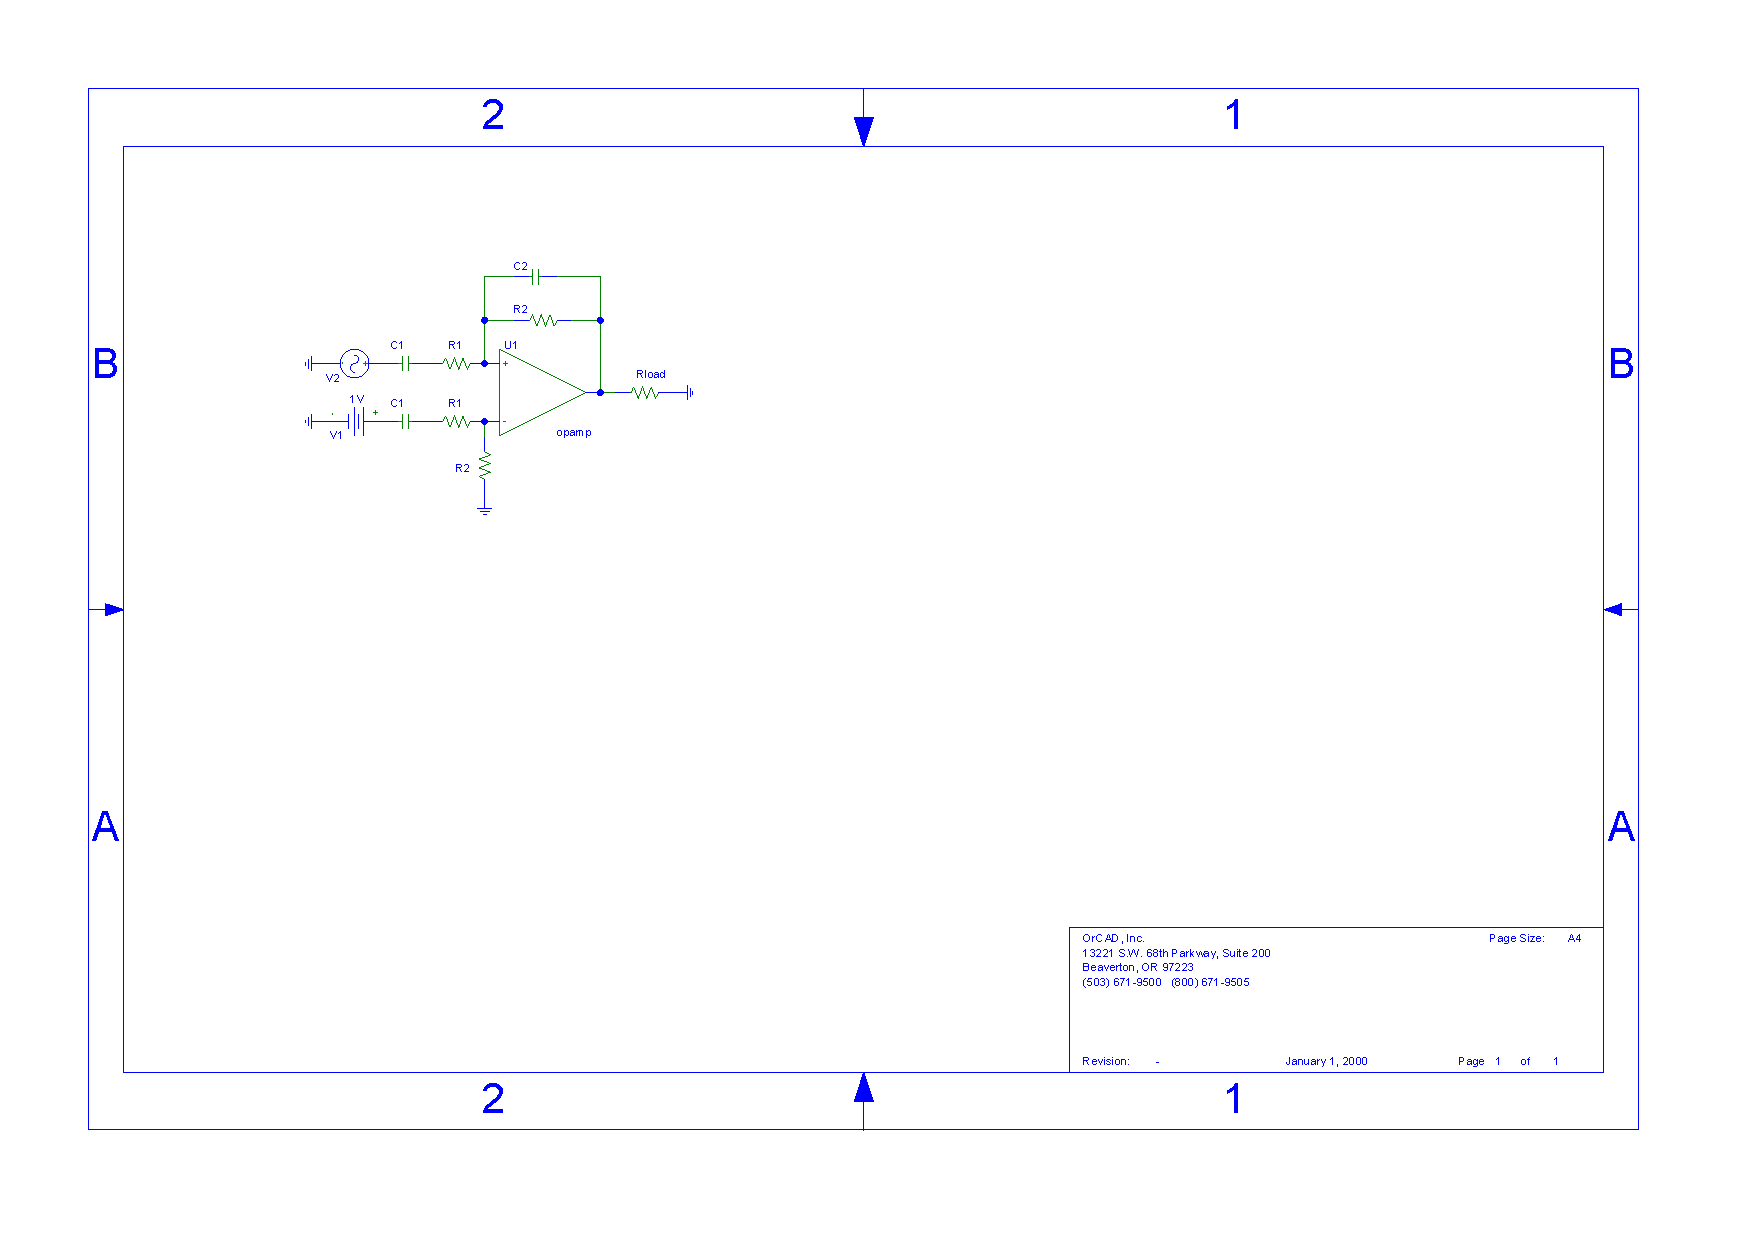
\includegraphics[width=0.6\textwidth, trim={5cm 12.29cm 17.6cm 4.3cm},clip]{opamp-dif2.pdf}
		%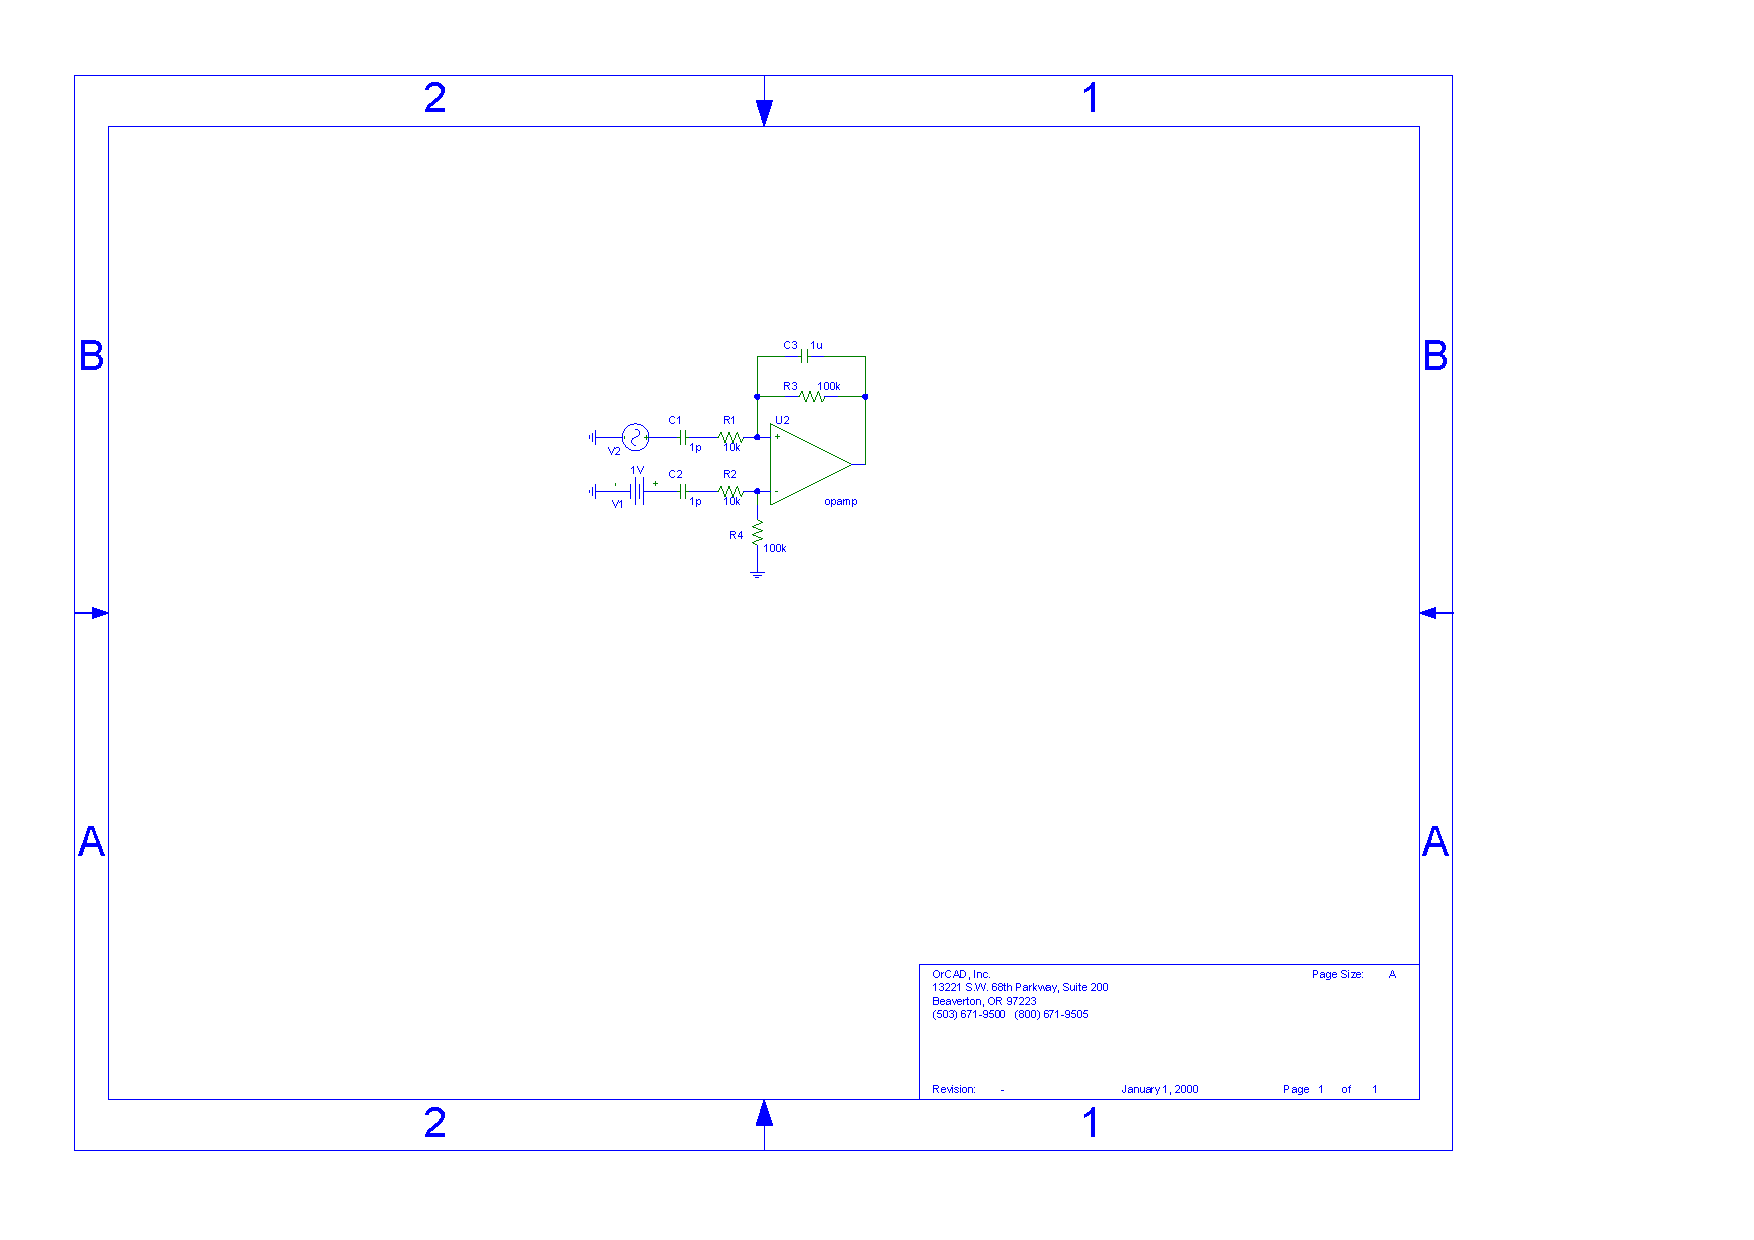
\includegraphics[width=0.5\textwidth, trim={9.5cm 11.2cm 15cm %5.76cm},clip]{opamp-dif.pdf}
		\legend{Fonte: Próprios autores}
	\end{figure}
	
	De acordo com as tabelas \ref{tab_phy1} e \ref{tab_phy2}, o intervalo da frequência do \textit{clock} luminoso é de 200kHz até 120MHz. Deseja-se então  permitir a passagem dessas, limitando as frequências fora desse intervalo. Com o uso do passa baixas e passa altas da figura acima, pode-se realizar essa limitação adequando os resistores e capacitores do circuito.
	
	\begin{figure}[htb]
		\caption{\label{fig_frequenciacentral}Um gráfico em escala logaritmica mostrando a banda de passagem B, a frequência de corte inferior Fl, a frequência de corte superior Fh e a frequência central fo para um circuito passa faixas.}
		\centering
		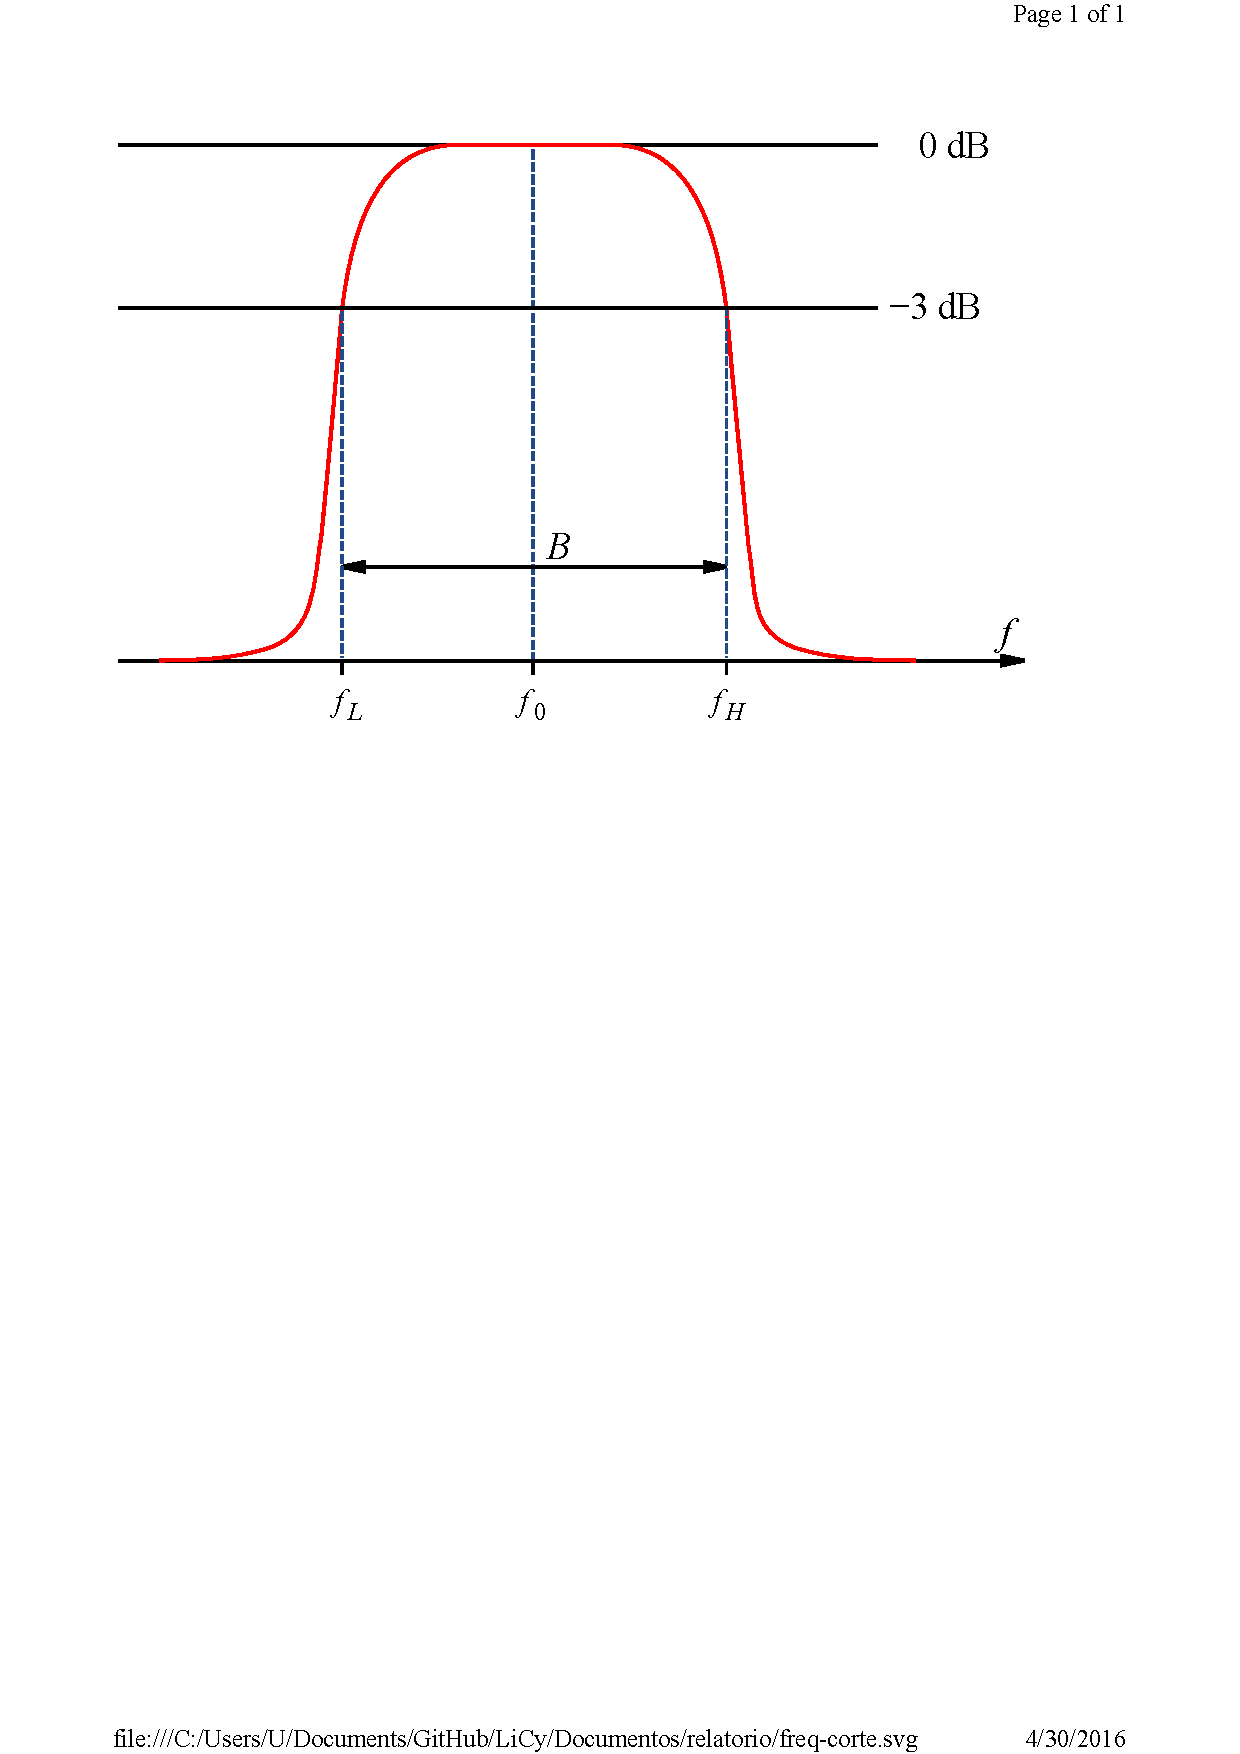
\includegraphics[width=0.5\textwidth, trim={4.5cm 17cm 3.3cm 2cm},clip]{freq-corte.pdf}
		\legend{Fonte: Inductiveload, Wikipedia}
	\end{figure}
	
	Deve-se levar em conta também o ganho do circuito, que é dado pela fórmula:
	
	\begin{equation}
	V_{out} = V_{in} \cdot \frac{R2}{R1}
	\end{equation}
	
	O cálculo da frequência de corte inferior do circuito é dado por: 
	
	\begin{equation} \label{eq:1}
	f_{ci} = \frac{1}{2 \cdot \pi \cdot R1 \cdot C1}
	\end{equation}
	
	No caso da frequência de corte superior, pode-se realizar o cálculo utilizando a fórmula abaixo:
	
	\begin{equation} \label{eq:2}
	f_{ci} = \frac{1}{2 \cdot \pi \cdot R2 \cdot C2}
	\end{equation}
	
	O cálculo da frequência central é feita pela \texttt{média geométrica} das frequências calculadas em \ref{eq:1} and \ref{eq:2} abaixo: 
	
	\begin{equation} \label{eq:3}
	f_{o} = \sqrt{f_{ci} \cdot f_{cs}}
	\end{equation}
	
	A banda de passagem do circuito é calculada pela subtração da frequencia de corte superior pela inferior:
	
	\begin{equation} \label{eq:4}
	BW = f_{cs} - f_{ci}
	\end{equation}
	
	Explicação de porque foi escolhido o circuito com ampop em modo diferencial para o projeto.
	
	% ---
	\subsubsection{Conversor Digital-Analógico}
	% ---	
	
	% ---
	\subsection{Microcontrolador}\label{hard-uc}
	% ---
	
	O microcontrolador escolhido foi o Raspberry Pi.

	% @TODO insira imagem do rasp aqui %
	
	Explicação do porquê foi escolhido Raspberry Pi: sistema linux, GPIO de fácil acesso, programação python
	
	% ---
	\subsubsection{Opções Consideradas}\label{uc-options}
	% ---
	
	Raspberry Pi, Galileo, 
	
	% ---
	\subsubsection{Tabela Comparativa}\label{uc-table}
	% ---
	
	% ---
	\subsection{FPGA}\label{hard-fpga}
	% ---
	
	FPGA (Field-Programmable Gate Array) é uma tecnologia que utiliza chips de silício reprogramáveis para obter circuitos customizáveis, latência a nível de hardware\footnote{muito muito rápido} e vazão muito alta\footnote{devido ao alto grau de paralelismo}. No projeto LiCy, como o fluxo de informações é muito alto (requisito de projeto de 1Gbps), é necessário realizar múltiplos processos ao mesmo tempo para lidar com os dados:
	
	\begin{itemize}  
		\item Recebimento/Transmissão de dados
		\item Cálculo de paridade
		\item Correção de erros\footnote{apenas para recebimento}
		\item (De)codificação de dados
	\end{itemize}
	
	\begin{table}[htbp]
		\caption{\label{tab_phy1} Modos de operação da camada PHY I de Li-Fi}
		
		\centering
		%  trim={<left> <lower> <right> <upper>} 
		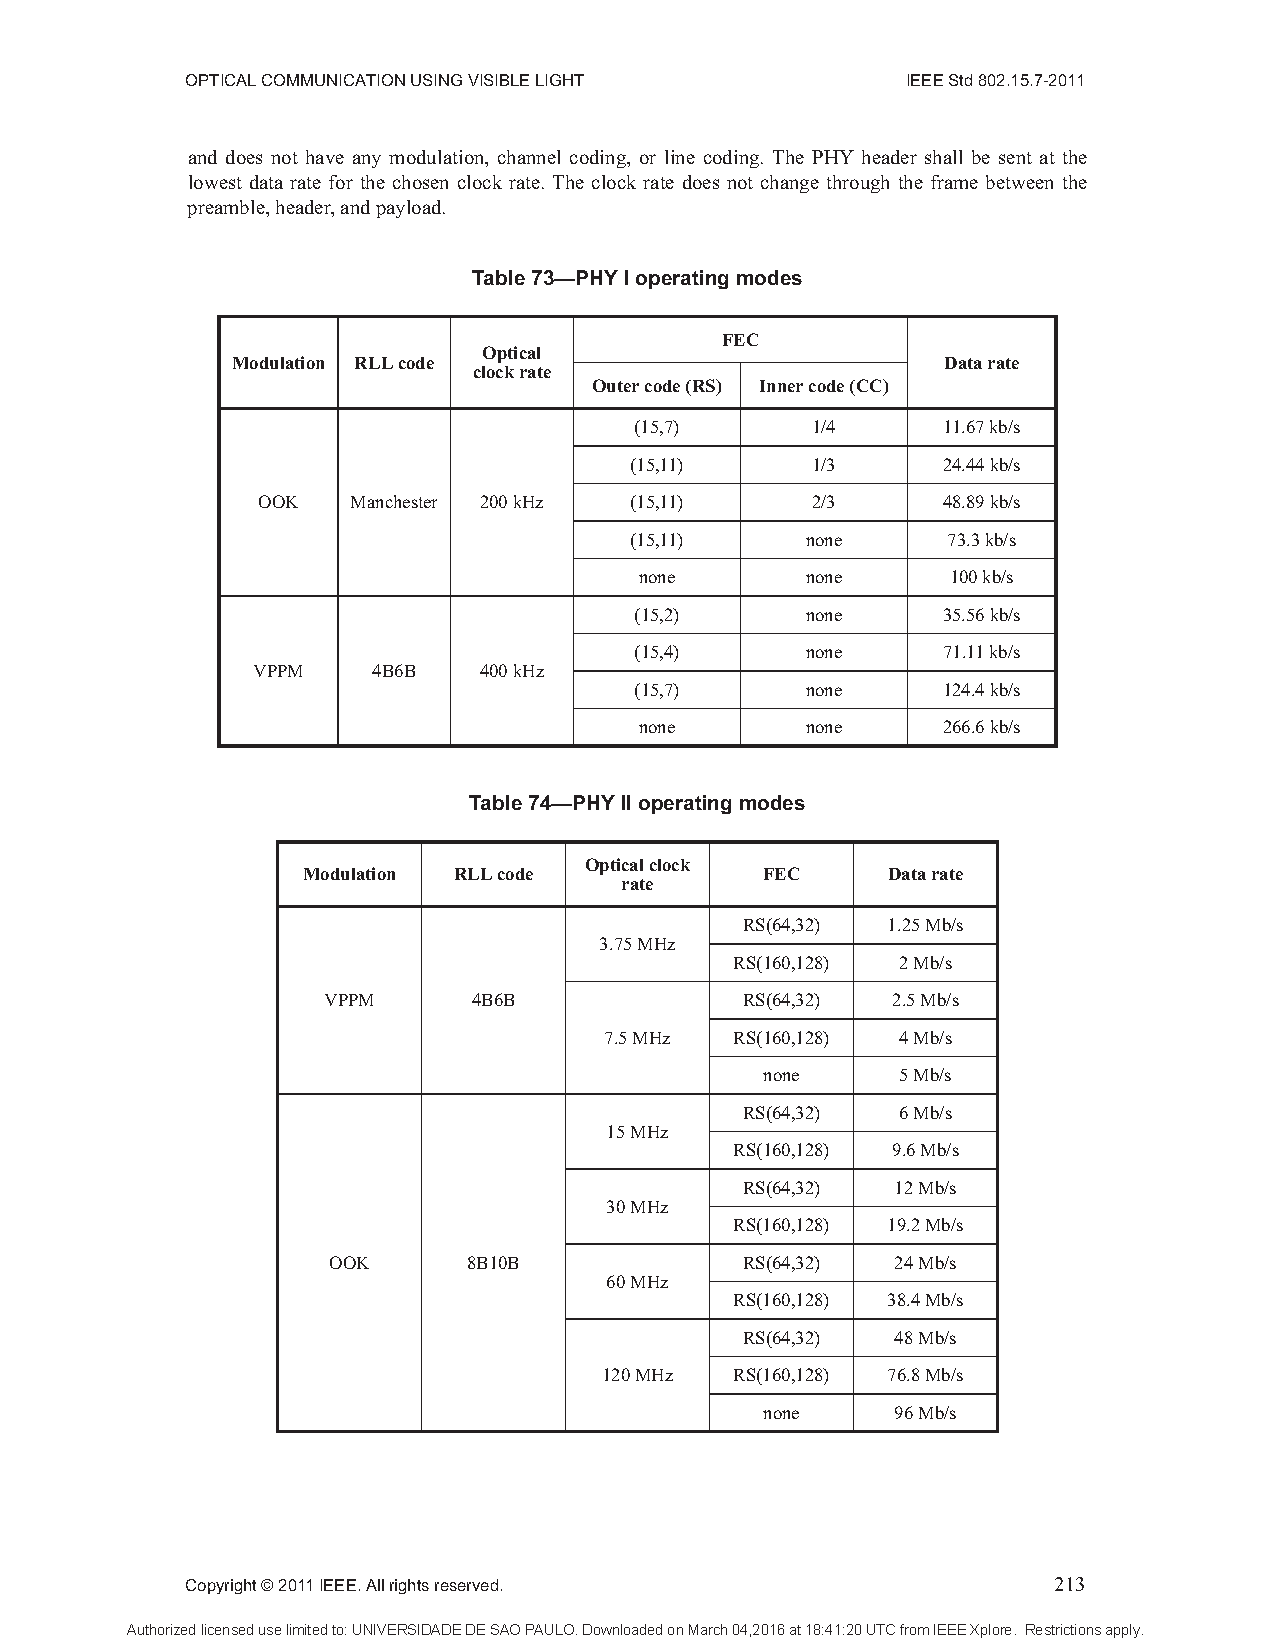
\includegraphics[clip, trim=37mm 151mm 36mm 51mm,  width=0.7\textwidth]{pag213.pdf}
		\legend{Fonte: IEEE 802.15.7}
	\end{table}
	
	\begin{table}[htbp]
		\caption{\label{tab_phy2} Modos de operação da camada PHY II de Li-Fi}
		\centering
		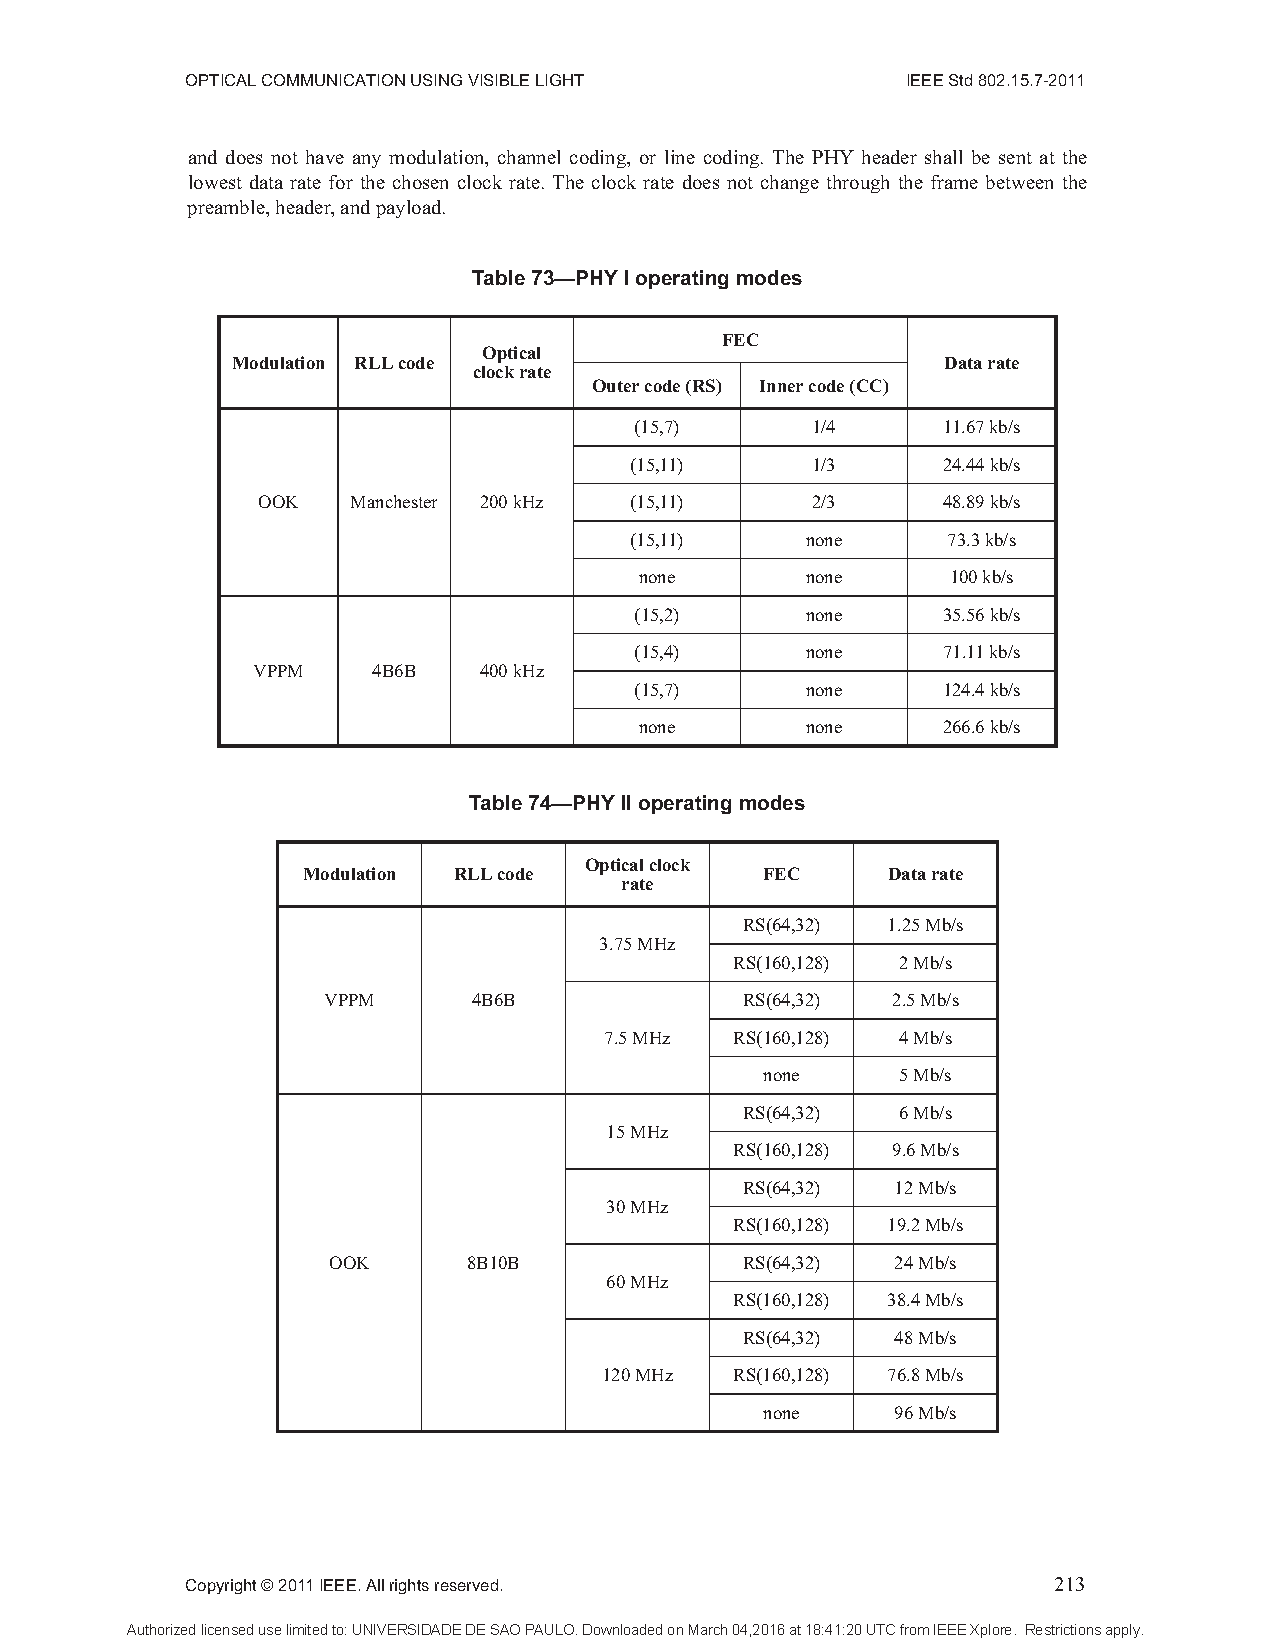
\includegraphics[clip, trim=46.55mm 36.79mm 46.74mm 142.30mm,  width=0.7\textwidth]{pag213.pdf}
		\legend{Fonte: IEEE 802.15.7}
	\end{table}
	
	Essa tecnologia é ideal para criar protótipos de circuitos digitais. Existe neste caso a facilidade de mudar o arranjo de componentes e vias de dados, bem como a possibilidade de simulá-los e depurá-los antes mesmo de gravar as configurações no hardware. Estes são elementos chave para a criação de um ambiente controlado, para testar as funcionalidades do produto desenvolvido. Sendo assim, um dos fatores que mais motivou a escolha dessa tecnologia neste projeto.
	
	O projeto de uma FPGA possui características que anteriormente estavam associadas a sistemas baseados em processadores. Uma delas é o uso de ferramentas e interfaces de alto nível, usando diagramas de bloco representando comportamentos e linguagens de descrição de hardware (na sigla em inglês, HDL), que no entanto diferem em muito de linguagens de programação como C. 
	
	A principal vantagem do uso de uma FPGA em relação a microcontroladores está na independência das operações de processamento, que por estarem em circuitos paralelos não precisam dividir recursos, como um mesmo núcleo por exemplo. Entretanto, o alto grau de paralelismo pode resultar em maiores desafios como garantir o sincronismo e lidar com inconsistência de dados no nível de circuito. Ainda assim, é preferível neste projeto lidar com esses desafios para se beneficiar do ganho em latência e vazão de dados.

	% ---
	\section{Software}\label{sec-software}
	% ---
	
	Explica as escolhas feitas no aspecto do software do projeto.
	
	% ---
	\subsection{VHDL}\label{soft-vhdl}
	% ---
	
	Explicação do porquê foi escolhido VHDL
	
	% ---
	\subsubsection{Opções Consideradas}\label{vhdl-options}
	% ---
	
	Explicação de quais foram as opções consideradas.
	
	% ---
	\subsubsection{Tabela Comparativa}\label{vhdl-table}
	% ---
	
	Tabela de opções consideradas.
	
	% ---
	\subsection{Quartus}\label{soft-quartus}
	% ---
	
	Explicação do porquê foi escolhido Quartus
	
	% ---
	\subsubsection{Opções Consideradas}\label{quartus-options}
	% ---

	
	% ---
	\subsubsection{Tabela Comparativa}\label{quartus-table}
	% ---
	
	
	% ---
	\subsection{Android}\label{soft-android}
	% ---
	
	Explicação do porquê foi escolhido Android.
